\documentclass[11pt]{article}
\usepackage{epsf}
\usepackage{hyperref}
\usepackage{graphicx}
\usepackage{subfigure}
\usepackage[margin=2.5cm]{geometry}
\usepackage{amsmath}
\usepackage{footnote}
\usepackage[bottom]{footmisc}
\usepackage[singlelinecheck=false]{caption}
\usepackage{caption}
\usepackage{amsthm}
\usepackage{enumitem}
\usepackage{graphics}
\usepackage{float}
\usepackage{amssymb}
\usepackage{natbib}
\usepackage{lscape}
\usepackage{array}
\textheight=8.7in
\usepackage{setspace}
\usepackage{verbatim}
\usepackage{multirow}

\def\threedigits#1{%
  \ifnum#1<100 0\fi
  \ifnum#1<10 0\fi
  \number#1}

\topmargin=0.1in \oddsidemargin=-0.1cm \evensidemargin=-0.1cm

\paperheight=11in \paperwidth=8.5in \marginparwidth=0in

\marginparsep=0in \textwidth=6.5in \headheight=0in \headsep=0in

\onehalfspacing
\def\argmax{\mathop{\rm arg\,max}}
%\usepackage{xspace,epsfig,subfig}
\newtheorem{theorem}{Theorem}
\newtheorem{lemma}{Lemma}
\newtheorem{claim}{Claim}
\newtheorem{proposition}{Proposition}
\newtheorem{definition}{Definition}
\newtheorem{corollary}{Corollary}
\newenvironment{sketch}{\noindent\emph{Proof Sketch:}}{$\quad \Box$}
%\newenvironment{proof}{\noindent\emph{Proof:}}{$\quad \Box$}

\bibpunct{(}{)}{;}{a}{,}{,}

\newcommand{\CV}{\operatorname{CV}}
\newcommand{\E}{\operatorname{E}}
\newcommand{\dataX}{\mathfrak{X}}
\newcommand{\Xtrain}{X_{\text{train}}}
\newcommand{\Ytrain}{Y_{\text{train}}}
\newcommand{\Xtest}{X_{\text{test}}}
\newcommand{\Ytest}{Y_{\text{test}}}
\newcommand{\hGX}{\hat G^{X}}
\newcommand{\hGY}{\hat G^{Y}}
\newcommand{\bpi}{\bar \pi}
\newcommand{\bmuX}{\bar \mu^{X}}
\newcommand{\bmuY}{\bar \mu^{Y}}
\newcommand{\sA}{\mathcal{A}}
\newcommand{\sbA}{\mathcal{\bar A}}
\newcommand{\sC}{\mathcal{C}}
\newcommand{\sE}{\mathcal{E}}
\newcommand{\sN}{\mathcal{N}}
\newcommand{\sX}{\mathcal{X}}

\begin{document}
\title{Estimating the number of clusters using Cross Validation}
\author{Wei Fu \qquad Patrick O. Perry \\\\ New York University}
\date{}
\maketitle
\begin{abstract}
Many clustering methods, including K-means, require the user to specify the number of clusters as an input parameter. A variety of methods have been devised to choose the number of clusters automatically, but they often rely on strong modeling assumptions. We propose a data-driven approach to estimate the number of clusters based on a novel form of cross-validation. This differs from ordinary cross-validation, because clustering is fundamentally an unsupervised learning problem. Simulation and real data analysis results show that our proposed method outperforms existing methods, especially in high-dimensional settings with heavy-tailed data.
\end{abstract}

\section{Introduction}
As a main task of exploratory data analysis, clustering organizes unlabeled observations into groups such that observations in same group are more similar compare to those in different group. Clustering is an important topic in unsupervised learning because it can reveal the internal structure of data through grouping, segment the data through partitioning and summarize data for other purposes such as dimension reduction. It has being widely used in various fields such as psychology, biology, statistics and machine learning including pattern recognition, image segmentation etc.\\

After being proposed more than $50$ years, $K$-mean remains one of the most
popular and widely used clustering algorithms \citep{jain2010data}. Like many
other clustering methods, $K$-mean requires an input parameter $k$, the number
of clusters, to be specified by the user. Automatically and quantitatively
deciding such parameter is important and yet unsolved problem
\citep{fujita2014non}. Various methods have been proposed to tackle this
difficulty. One ad hoc approach is to explore the relationship between $W_k$
(within-cluster dispersion) and the number of cluster $k$ for a certain
clustering method such as $K$-mean. Since $W_k$ decreases as $k$ increases,
one usually find the ``elbow" of curve $W_k$ \textsl{VS} $k$ as the
appropriate number of clusters. The example on the top row of Figure
\ref{fig:elbow} demonstrates such approach for data with $k=4$, where the
``elbow" point indeed reveals the true number of clusters. This is based on
the idea that under partitioning data set has more impact than over
partitioning data set in terms of $W_k$. However, locating the ``elbow" point
is somewhat subjective and sometimes is not appropriate to select the optimal
$k$. The second example on the bottom row of Figure \ref{fig:elbow} shows a  situation where there is no clear choice of the ``elbow" point -- both $k=2$ and $k=3$ can be viewed as the ``elbow" point. What's more, the true $k=4$ can never be selected as the optimal $k$ using such approach in this case since it can hardly be viewed as the ``elbow" of the curve.

\begin{figure}
\centering
\begin{minipage}{\linewidth}
  \begin{minipage}{0.45\linewidth}
    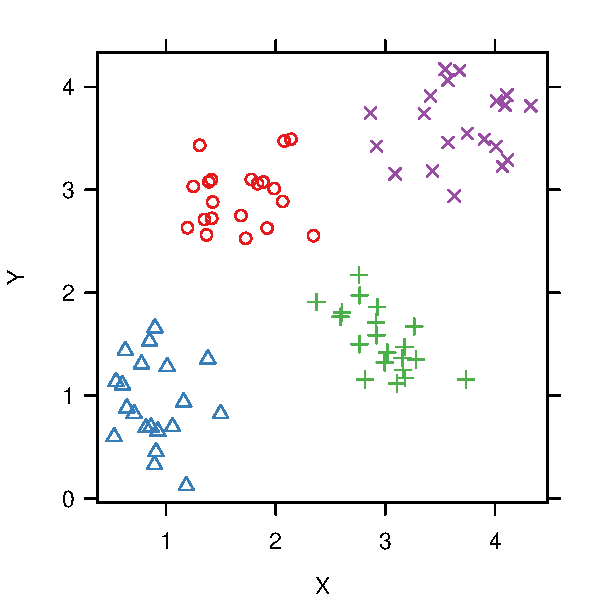
\includegraphics[width=\linewidth]{demo/elbow/correct-data.pdf}
  \end{minipage}
  \hspace{0.05in}
  \begin{minipage}{0.45\linewidth}
    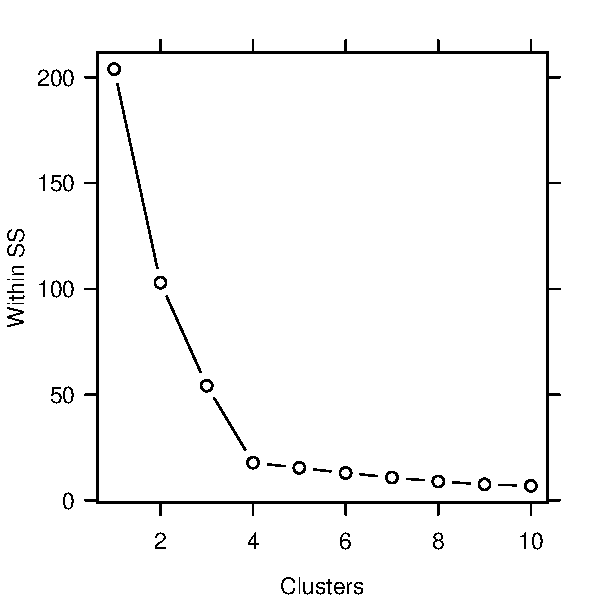
\includegraphics[width=\linewidth]{demo/elbow/correct-withinss.pdf}
  \end{minipage}
\end{minipage}
\begin{minipage}{\linewidth}
  \begin{minipage}{0.45\linewidth}
    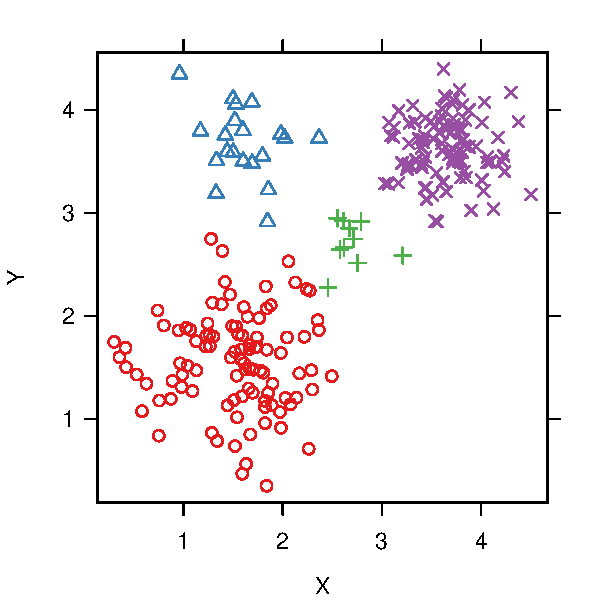
\includegraphics[width=\linewidth]{demo/elbow/incorrect-data.pdf}
  \end{minipage}
  \hspace{0.05in}
  \begin{minipage}{0.45\linewidth}
    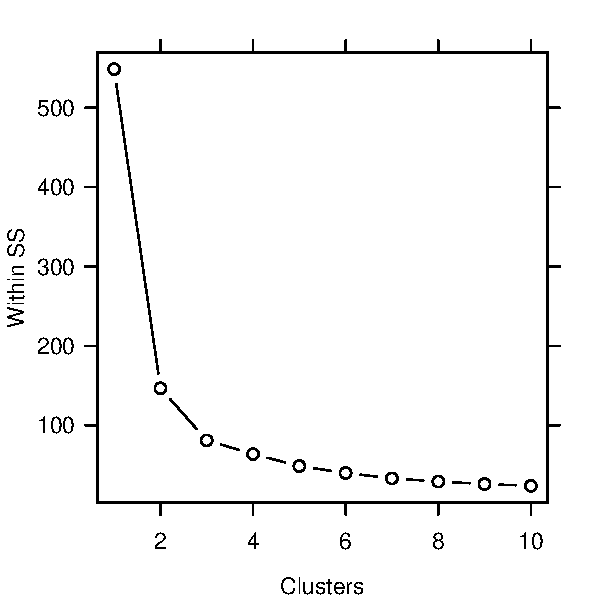
\includegraphics[width=\linewidth]{demo/elbow/incorrect-withinss.pdf}
  \end{minipage}
\end{minipage}
\caption{Left panels show the $(X,Y)$ data points; right panels
  show the corresponding values of the within-cluster sum of squares $W_k$
plotted against the number of clusters, $k$.}
\label{fig:elbow}
\end{figure}


Recently, there are several new proposals to find the $k$ automatically. Gap statistics \citep{tibshirani2001estimating} estimates $k$ by comparing the change in within-cluster dispersion with that expected under an appropriate reference null distribution. Specifically, the graph of $log(W_k)$ is compared with its expectation under an appropriate null reference distribution of the data. The value of $k$ associated with the largest gap between $log(W_k)$ and the reference curve is selected as optimal $k$. \cite{sugar2003finding} proposed an approach which finds the number of clusters based on distortion, a quantity that measures the average distance, per dimension. It's backed by a rigorous theoretical justification based on information-theoretic ideas.   \cite{fraley2002model}'s Model-based method employs the EM algorithm to estimate the parameters in Gaussian mixture model, and select the best model ($k$) using BIC criterion. Stability-based criterion is also proposed to locate the best $k$ by some authors such as \cite{ben2001stability}, \cite{wang2010consistent} and \cite{fang2012selection}. \cite{chiang2010intelligent} provides a nice review of existing methods for finding the right $k$ in published literature. \\

Most existing methods are either model based method requires strong parameter assumptions or ad hoc method utilizes within-cluster dispersion. Although many view selecting the number of clusters as a model selection problem, very few approaches this problem from the prediction point of view. Select model with smallest prediction error via cross-validation is one of the simplest and most widely used model selection techniques in supervised learning. The lack of true class (label) in data set makes the adoption of cross-validation into unsupervised leaning problem difficult. Perhaps the only exception is \cite{tibshirani2005cluster}, which selects the optimal $k$ by prediction strength. The strategy is to first cluster the test data and training data into $k$ clusters respectively. Then, for each pair of observations that are assigned to the same test cluster, algorithm determines whether they are also assigned to the same cluster based on the training centers. The intuition here is, if $k=k_0$, the true number of clusters, then the $k$ training set clusters will be similar to the $k$ test clusters, and hence will predict them well. However, a specifically defined prediction error measure is used in such procedure, which is quite different from the one commonly used in cross-validation procedure in supervised learning. Therefore the well understood properties of cross-validation procedure in supervised learning cannot be carried over to the prediction strength method, makes the interpretation of its result difficult. \\

Our proposed method is a complete data-driven approach which doesn't rely on any parametric assumptions. Through novel form of partitioning data set, we are able to employing the cross-validation procedure in clustering exactly the same way as in supervised learning problem. Hence, it's easy for reader to understand the intuition behind our proposed method. Simulation and real data application shows the superior performance of our proposed method compare with existing methods in high-dimension settings and heavy-tailed data. Since the embedded cross-validation procedure is well understood, it also makes our method potentially easily to be extended in future study. 
 

\section{Cross-validation for selecting the number of clusters}

Cross-validation is commonly used for model selection in supervised learning
problems.  In these settings, the data comes in the form of $N$
predictor-response pairs, $(X_1, Y_1), \dotsc, (X_N, Y_N)$, with $X_i \in
\mathbb{R}^{p}$ and $Y_i \in \mathbb{R}^{q}$.  The data can be represented as
a matrix with $N$ rows and $p + q$ columns.  We partition the data into $K$
hold-out ``test'' subsets, with $K$ typically chosen to be $5$ or $10$.  For each
``fold'' $r$ in the range $1, \dotsc, K$, we permute the rows of the data
matrix to get $\dataX$, a matrix with the $r$th test subset as its trailing
rows.  We partition $\dataX$ as
\[
  \dataX =
  \begin{bmatrix}
    \Xtrain & \Ytrain \\
    \Xtest  & \Ytest
  \end{bmatrix}.
\]
We use the training rows $[ \Xtrain\ \Ytrain ]$ to fit a regression model
$\hat Y = \hat Y(X)$, and then evaluate the performance of this model on the
test set, computing the cross-validation error $\|\Ytest - \hat Y(\Xtest)\|^2$
or some variant thereof.  We choose the model with the smallest
cross-validation error, averaged over all $K$ folds.


In unsupervised learning problems like factor analysis and clustering, the
features of the observations are not naturally partitioned into ``predictors''
and ``responses'', so we cannot directly apply the cross-validation procedure
described above.  For factor analysis, there are at least two versions of
cross-validation.  \citet{wold78cross} proposed a ``speckled'' holdout, where
in each fold we leave out a subset of the elements of the data matrix.  Wold's
procedure works well empirically, but does not have any theoretical support,
and it requires a factor analysis procedure that can handle missing data.
\citet{owen2009bi} proposed a scheme called ``bi-cross-validation'' wherein
each fold designates a subset of the data matrix columns to be response and a
subset of the rows to be test data.  This generalized a procedure due to
\citet{gabriel2002biblot}, who proposed holding out a single column and a
single row at each fold.  Owen and Perry proved that this procedure is
self-consistent, in the sense that it performs the correct model selection in
the absence of noise, and \citet{perry2009cross} provided more theoretical
support.


In this report, we extend the Wold and Gabriel methods to the clustering
problem, specifically to choose an appropriate number of clusters for a
dataset.  We prove that the Gabriel method is self-consistent, and we analyze
some of its properties in the presence of noise.  We compare these methods to
state-of-the-art algorithms, and show that both are competitive.



%% [POP] This paragraph doesn't fit into the section.  Maybe put it in the introduction?
%% 
%% Cross-Validation technique, one of the most commonly used and popular model
%% selecting method in supervised learning, can not be used naively in
%% unsupervised learning context. Since prediction error of new observation is
%% calculated by its distance to the nearest cluster center, more cluster centers
%% means much tighter fit to the feature space, and hence smaller distance
%% (prediction error) of observation to its nearest cluster center. This holds
%% even when the prediction is evaluated on an independent test set
%% \citep{hastie2009elements}. Therefore, CV prefers larger $k$ if we do the CV
%% naively.




We now give the details of how to implement
the Gabriel cross-validation to locate the optimal cluster number $k$. The
Wold cross-validation algorithm is described in Appendix $A$.


\subsection*{Gabriel CV algorithm}

We are given a data matrix with $N$ rows and $P$ columns.  In each fold of
cross-validation, we permute the rows and columns of the data matrix and then
partition the rows and columns as $N = n + m$ and $P = p + q$ for 
non-negative integers $n$, $m$, $p$, and $q$.  We treat the first $p$
columns as ``predictors'' and the last $q$ columns as ``responses'';
similarly, we treat the first $n$ rows as ``training'' and the last $m$ rows
as ``test''.  In block form, the permuted data matrix is
\[
  \dataX
  =
  \begin{bmatrix}
    \Xtrain & \Ytrain \\
    \Xtest  & \Ytest
  \end{bmatrix},
\]
where
$\Xtrain \in \mathbb{R}^{n \times p}$,
$\Ytrain \in \mathbb{R}^{n \times q}$,
$\Xtest \in \mathbb{R}^{m \times p}$,
and
$\Ytest \in \mathbb{R}^{m \times q}$.


Given such a partition of $\dataX$, we perform four steps for each value of
$k$, the number of clusters:
\begin{enumerate}
  \item \label{step:gabriel-cluster}
    \textbf{Cluster:}
    Cluster $Y_{1}, \dotsc, Y_n$, the rows of $\Ytrain$, yielding the
    assignment rule $\hGY : \mathbb{R}^q \to \{ 1, \dotsc, k \}$ and the
    clusters means $\bmuY_1, \dotsc, \bmuY_k$.  Set $\hGY_i = \hGY(Y_i)$ to
    be the assigned cluster for row $i$.

  \item \label{step:gabriel-classify}
    \textbf{Classify:}
    Take $X_{1}, \dotsc, X_n$, the rows of $\Xtrain$ to be predictors,
    and take $\hGY_1, \dotsc, \hGY_n$ to be corresponding class labels.  Use
    the pairs $\{ (X_i, \hGY_i) \}_{i=1}^{n}$ to train a classifier
    $\hGX : \mathbb{R}^p \to \{ 1, \dotsc, k \}$.

  \item \label{step:gabriel-predict}
    \textbf{Predict:}
    Apply the classifier to $X_{n+1}, \dotsc, X_{n+m}$, the rows of
    $\Xtest$, yielding predicted classes $\hGX_i = \hGX(X_i)$ for
    $i = n+1, \dotsc, n+m$.  For each value of $i$ in this range, compute
    predicted response $\hat Y_i = \bmuY(\hGX_i)$, where
    $\bmuY(g) = \bmuY_g$.

  \item \label{step:gabriel-evaluate}
    \textbf{Evaluate:}
    Compute the cross-validation error
    \[
      \CV(k) = \frac{1}{m} \sum_{i=n+1}^{n+m} \|Y_i - \hat Y_i\|^2,
    \]
    where $Y_{n+1}, \dotsc, Y_{n+m}$ are the rows of $\Ytest$.
\end{enumerate}
\noindent
In principle, we could use any clustering and classification methods in
steps~\ref{step:gabriel-cluster} and~\ref{step:gabriel-classify}.  In this
report, we use $k$-means as the clustering algorithm and linear discriminant
analysis (LDA) as the classification procedure.


To choose the folds, we randomly partition the rows and columns into $K$ and
$L$ subsets, respectively.  Each fold is indexed by a pair $(r,s)$ of
integers, with $r \in \{1, \dotsc, K\}$ and $s \in \{1, \dotsc, L\}$.  Fold
$(r,s)$ treats the $r$th row subset as ``test'', and the $s$th column subset
as ``response''.  Following \citet{owen2009bi}, we take $K = L = 2$.  For the
number of clusters, we select the value of $k$ that minimizes the average of
$\CV(k)$ over all $K \times L$ folds.



\section{Theoretical justification of Gabriel CV method}

This section gives the self-consistency proof of the proposed Gabriel method. What's more, its asymptotic property under suitable condition will be shown in this section in order to give the idea of why the Gabriel CV method works.\\

Because K-means algorithm is a key part in the proof below, it's convenient to have a review of K-means here:\\
Given a set of observations $\mathbf{X} = (x_1,...,x_n)$, and the number of clusters $K$, K-means' goal is to minimize the within cluster dispersion. That is, find the partition $\mathbb{P}_K$ of $\mathbf{X}$, where $\mathbb{P}_K(\mathbf{X})= (p_1,p_2,...,p_K)$, such that
\[	\underset{\mathbb{P}_K}{\operatorname{argmin}} \sum^K_{i=1}\sum_{x \in p_i } ||x-\hat{\mu}_i||^2\]
where $\hat{\mu}_i$ is the sample mean of $p_i$.
\subsection{Self-Consistency}
Same as in section $2$, let the data set $\mathbf{X} \in \mathbb{R}^{n \times p}$ been partitioned as 
 \[ 
 \begin{pmatrix}
\mathbf{X}^L_{train} & \mathbf{X}^R_{train}\\
  \mathbf{X}^L_{test}  & \mathbf{X}^R_{test}\\
  \end{pmatrix}
 \]
\subsection*{Assumptions}
\begin{enumerate}[label={Assumption},leftmargin=*]
\item $1.$ There are $K$ true centers $(\mu_1,...,\mu_K)$ where $\mathbf{X}$ generated from
\item $2.$ The $K$ partitioned centers $(\mu^L_1,...,\mu^L_K)$ are all distinct in $L$ dimensions: $||\mu^L_i-\mu^L_j|| \neq 0$ for any $i \neq j$; $(\mu^R_1,...,\mu^R_K)$ are all distinct in $R$ dimensions
\item $3.$ The training set contains at least one member of each cluster
\item $4.$ The test set contains at least one member of each cluster
\item $5.$ There is no noise, so that $$x_i = \mu \left(c_i\right) \in \{\mu_1,...,\mu_K\} $$ and $$\mu \left(c_i\right) = \mu_j \hspace{0.2in} \text{iff} \hspace{0.2in} c_i = j$$ where $c_i$ is the true cluster for observation $i$, which implies $$x^L_i = \mu^L\left(c_i\right) \in \{\mu^L_1,...,\mu^L_K\},\hspace{0.2in} x^R_i = \mu^R\left(c_i\right) \in \{\mu^R_1,...,\mu^R_K\}$$
\end{enumerate}
 
\begin{proposition}
	If assumptions $1, 2, 3, 5$ hold, then there exists a classification method works perfectly in case of ($k \leq K$): the re-substitution error is $0$. That is, for $\forall x_i \in \mathbf{X}_{train}$ prediction on $x^L_i$ always correctly predict cluster where $x^R_i$ is in.
\end{proposition}

\begin{theorem}
Given assumptions $1-5$, $ E\left(Error_k\right) > 0$ for $k<K$ and  $ E\left(Error_k\right) = 0$ for $k=K$. Hence if $k \leq K$, the Gabriel algorithm selects $k=K$ with probability $1$.
\end{theorem}
\noindent
Not that $k > K$ is not considered here because there are only $K$ unique points in $\mathbf{X}$. K-means will not work for parameter which is larger than the number of unique points in data $\mathbf{X}$.\\\\ 
\noindent
The proof of above theorem follows from following two lemmas:
\begin{lemma}
	If the assumptions of Theorem $1$ hold, then when $k<K$, the CV Error $>0$
\end{lemma}
\begin{proof}
	It is sufficient to prove that when $k<K$,  $Error_k>0$. By the definition of $Error_k$,
\begin{equation}
Error_k = \sum^k_{j=1} \sum_{g_j = \hat{g} \left(x^L_i\right)} ||\hat{\mu}^R \left(g_j\right) - x^R_i||^2
\end{equation}
	where $\hat{\mu}^R \left(g_j\right)$ is the center of cluster $g_j$ returned from K-means. By assumption $4$, test set contains at least one member of each cluster. Since there are $K$ true centers, and by assumption $5$, $x_i = \mu \left(c_i\right) \in \{\mu_1,...,\mu_K\} $, test set contains $K$ centers. It means there are $K$ distinct $x^R_i \left(=\mu^R \left(c_i\right)\right)$ in $\mathbf{X}^R_{test}$ set by assumption $2$. However, in equation $(1)$, there are only $k$ distinct $\hat{\mu}^R \left(g_j\right)$.  Because $k < K$, it means not every element $||\hat{\mu}^R \left(g_j\right) - x^R_i||^2 = 0$ in equation $(1)$. Therefore,  $$Error_k = \sum^k_{j=1} \sum_{g_j = \hat{g} \left(x^L_i\right)} ||\hat{\mu}^R \left(g_j\right) - x^R_i||^2 > 0$$
\end{proof}
\begin{lemma}
	If the assumptions of Theorem $1$ hold, when $k=K$, the CV Error $=0$
\end{lemma}
\begin{proof}
	It's sufficient to show that when $k=K$, $Error_k=0$. By assumption $3$ and $5$, training set contains $K$ centers. Which also implies $\mathbf{X}^R_{train}$ contains $K$ distinct $x^R_i$ $(\mu^R_1,...,\mu^R_K)$. When apply K-means on $\mathbf{X}^R_{train}$ with parameter $K$, the unique solution of 
	\[ \underset{\left(\hat{\mu}^R\left(g_1\right),...,\hat{\mu}^R\left(g_K\right)\right)}{\operatorname{argmin}} \sum^K_{j=1} \sum_{g_j = \hat{g} \left(x^R_i\right)} ||\hat{\mu}^R \left(g_j\right) - x^R_i||^2 \]
	is 
\begin{equation}	
	\{\hat{\mu}^R \left(g_j\right) = \mu^R_j, j=1,...,K\}
\end{equation}	
with 
\begin{equation}	 
	\hat{g} \left(x^R_i\right) = \sum^K_{j=1} g_j \cdot I_{c_i = j}
\end{equation}	
Where $\hat{g} \left(x^R_i\right) \in  \mathcal{G}$ is the assigned cluster of $x^R_i$ by K-means. One can easily check that such solution is unique and above objective function attains its lower bound $0$.\\\\
By Proposition $1$, $\mathcal{C}$ has re-substitution error $0$, which means its prediction error is $0$ on $\mathbf{X}^L_{test}$ as $\forall x^L_i \in \mathbf{X}^L_{test}, x^L_i \in \mathbf{X}^L_{train}$ by assumption $1,3,5$. Hence the predicted cluster $\hat{g} \left(x^L_i\right)$ for $x_i$ is the correct one $\hat{g} \left(x^R_i\right)$, which determined by $x^R_i$. By equation $(3)$, we have $x^R_i = \mu^R \left(c_i\right) = \mu^R_j$ if $\hat{g} \left(x^L_i\right) = \hat{g} \left(x^R_i\right) = g_j$. Therefore,
\[ Error_K = \sum^K_{j=1} \sum_{g_j = \hat{g} \left(x^L_i\right)} ||\hat{\mu}^R \left(g_j\right) - x^R_i||^2 =  \sum^K_{j=1} \sum_{g_j = \hat{g} \left(x^L_i\right)} ||\hat{\mu}^R \left(g_j\right) - \mu^R_j||^2= 0\]
The last equation holds because of equation $(2)$.
\end{proof}

\begin{itemize}
	\item Proof of \textbf{Proposition} $1$.
	\begin{proof}
	To train classifier $\mathcal{C}$, we have training set $\left(\mathbf{X}^L_{train},\mathcal{G} \right) = \{\left(x^L_i,\hat{g} \left(x^R_i\right)\right), i =1,2,...,m\}$. By assumption $5$, $\forall i$ $x_i = \mu_j$, $j=1,2,...,K$ and $k \leq K$. Hence the training set has $K$ unique pairs $\{\left(\mu^L_j, \hat{g} \left(\mu^R_j\right)\right),j=1,2,...,K\}$, with $K$ unique $\mu^L_j$ by assumption $3$ and $k$ unique $\hat{g} \left(\mu^R_j\right)$. This is because each pair $(\mu^L_j,\mu^R_j)$ is unique by assumption $2$ and $\left(\mu^R_j,\hat{g} \left(\mu^R_j\right)\right)$ is unique since K-means assigns one and only one label to each $\mu^R_j$. Define the classifier $\mathcal{C}$ as following: \[ \mathcal{C}(x^L_i) = \sum^K_{j=1}\hat{g} \left(\mu^R_j\right) \cdot I_{\{c_i = j\}}  \] It's easy to see such classifier has re-substitution error $0$. 
	\end{proof}
	\item Proof of \textbf{Proposition} $1$ when the classifier is LDA.
	\begin{proof}
	Since Proposition $1$ is only used in Lemma $2$, therefore it's sufficient to prove it in case of $k = K$. Note that training set contains $K$ unique pairs $\{\left(\mu^L_j, \hat{g} \left(\mu^R_j\right)\right), j=1,2,...,K\}$, with $K$ unique $\mu^L_j$ and $K$ unique $\hat{g} \left(\mu^R_j\right)$ now, where $\mu^L_j, \hat{g} \left(\mu^R_j\right)$ has one-to-one correspondence, i.e.
\[ \left\lbrace\left(\mu^L_j,\hat{g} \left(\mu^R_j\right) \right), j=1,2,...,K\right\rbrace =  \left\lbrace\left(\mu^L_j, g_j \right), j=1,2,...,K\right\rbrace \]
By equation $(3)$.\\\\
Let the prior probability of class $g_j$ be $\pi_j, \hspace{0.05in} j=1,...,K$. By assumption $3$, $\pi_j > 0$. The class-conditional density of $X$ in class $\mathcal{G} = g_j$ is $$f_j\left(x_i\right) = \mathbb{P}\left( X=x_i | \mathcal{G} = g_j \right) $$ where $x_i \in \{\mu^L_1,...,\mu^L_K\}$ and $f_j\left(x_i\right)$ has multivariate Gaussian distribution
\[ f_j\left(x_i\right) = \frac{1}{(2\pi)^{p/2}|\Sigma_j|^{1/2}}e^{-\frac{1}{2}(x_i-\mu_j)^T\Sigma^{-1}_j(x_i-\mu_j)	}\]
LDA assumes a commom covariance matrix $\Sigma_j = \Sigma \hspace{0.1in} \forall j$.
The posterior probability is 
\[	\mathbb{P}\left( \mathcal{G} = g_j | X=x_i  \right)  = \frac{f_j\left(x_i\right) \pi_j}{\sum^K_{l=1}f_l\left(x_i\right) \pi_l}	\]
In practice, $\pi_j, \mu_j$ and $\Sigma$ are estimated from data by
 \begin{itemize}
 	\item  $\hat{\pi}_j = \frac{N_j}{N}$, where $N_j$ is the number of class-$g_j$ observation in training set and $N$ is the total observation in training set
 	\item  $\hat{\mu}_j = \sum_{c_i=j} x_i/N_j$ 
 	\item  $\hat{\Sigma} = \frac{1}{N-K} \sum^K_{j=1}\sum_{c_i=j} (x_i - \hat{\mu}_j )(x_i - \hat{\mu}_j )^T$
 \end{itemize}
In our case, $\hat{\mu}_j = \mu^L_j$ and $\hat{\Sigma}$ is zero matrix by construction. But in real case, the estimate of within-group covariance $\hat{\Sigma}$ is a positive-definite matrix. We therefore assume $\hat{\Sigma}$ to be any positive-definite matrix. Also, we assume the observations in training set are evenly distributed across all class, i.e. $\pi_j$ is a positive constant for all $j = 1,...,K$ \\\\   
LDA predicts class for each $x_i = \mu^L(c_i)\in \{\mu^L_1,...,\mu^L_K\}$ by maximizing the posterior probability
\begin{align}
     \hat{\mathcal{G}}(x_i) & = \underset{g_j}{\operatorname{argmax}}\hspace{0.05 in} \mathbb{P}\left( \mathcal{G} = g_j | X=x_i  \right)  \nonumber   \\ 
     & = \underset{g_j}{\operatorname{argmax}}\hspace{0.05 in} f_j\left(x_i\right) \pi_j \nonumber \nonumber  \\
     & = \underset{g_j}{\operatorname{argmax}}\hspace{0.05 in} f_j\left(x_i\right) \nonumber  \nonumber  \\    
     & = \underset{g_j}{\operatorname{argmax}}\hspace{0.05 in}  \frac{1}{(2\pi)^{p/2}|\hat{\Sigma}|^{1/2}}e^{-\frac{1}{2}(x_i-\mu^L_j)^T\hat{\Sigma}^{-1}(x_i-\mu^L_j)	} \nonumber  \\  
     &=  \underset{g_j}{\operatorname{argmin}}\hspace{0.05 in} (x_i-\mu^L_j)^T\hat{\Sigma}^{-1}(x_i-\mu^L_j) \nonumber   \\  
     &= \sum^K_{j=1} g_j \cdot I_{c_i = j}
\end{align}
The last equation holds because $\hat{\Sigma}$ is assumed to be positive-definite, so is its inverse  $\hat{\Sigma}^{-1}$. Hence $(x_i-\mu^L_j)^T\hat{\Sigma}^{-1}(x_i-\mu^L_j) >0$ for any non-zero vector $(x_i-\mu^L_j)$. The lower bound $0$ is attained only when $(x_i-\mu^L_j)$ is a zero vector, which is only possible when $x_i=\mu^L(c_i) = \mu^L_j$, i.e. $c_i = j$ by assumption $2$ and $5$. \\\\
Because the RHS of equation $(4)$ coincide with RHS of equation $(3)$, the proof is complete.
\end{proof}
\end{itemize}

\subsection{Single Cluster With Noise}

Here, we show that Gabriel Cross-Validation is consistent when the data come
from a single cluster; the algorithm picks $k = 1$ with probability tending to
$1$ as the number of rows in the data matrix $\dataX$ increase.


Our proof relies on results from \citet{pollard1981strong}, who analyzed
$k$-means and showed that the within-cluster sum of squares converges to a
population quantity.  Specifically, for any finite set $A \subset
\mathbb{R}^d$ and probability measure $P$ supported on $\mathbb{R}^d$, define
the population within-cluster sum of squares as
\[
  W(A, P) = \int \min_{a \in A} \|x - a\|^2 P(dx).
\]
Define
\(
  \sA_k
    =
    \{ A \subset \mathbb{R}^d : \text{$A$ contains $k$ or fewer points} \}
\)
and set
\(
  m_k(P) = \inf_{A \in \sA_k}  W(A, P). % : \text{$A$ contains $k$ or fewer points} \}.
\)
Suppose that $X_1, \dotsc, X_n$ are independent draws from $P$, and if $P_n$
is the empirical measure formed by placing mass $1/n$ on each $X_i$.  Let
$A_n$ be a set minimizing $W(A_n, P_n)$.  Pollard gave conditions for $A_n$ to
converge to the minimizer of $W(\cdot, P)$.  His main theorem assumes that the
minimizer of $W(\cdot, P)$ is unique, which is too strong for our purposes
(this fails, for example, with a bivariate normal distribution with identity
covariance whenever $k \geq 2$).  It is straightforward to generalize his
result to cases with multiple maximizers.  To do so, we will need the
following three lemmas.  The proofs of these lemmas are modifications of
arguments given in Sections~3 and~4 of Pollard's article.




\begin{lemma}[Continuity]\label{lem:pollard-continuous}\label{lem:pollard-last}
If $\int \|x\|^2 P(x) < \infty$, then the map $A \mapsto W(A, P)$ is
continuous on $\sA_k$ with respect to the topology induced by the Hausdoff
metric $H(\cdot, \cdot)$, defined for compact subsets $A, B$ of $\mathbb{R}^d$
by $H(A,B) < \delta$ if and only if every point of $A$ is within Euclidean
distance $\delta$ of at least one point of $B$, and vice versa.
\end{lemma}
\begin{proof}
This is a slight extension of the argument given at the end of Pollard's
Section~4.  If $A, B \in \sA_k$ and $H(A, B) < \delta$, then for each $b \in
B$ there exists an $a(b) \in A$ such that $\|b - a(b)\| < \delta$.  Then
\begin{align*}
  W(A, P) - W(B, P)
    &= \int \min_{a \in A} \|x - a\|^2 - \min_{b \in B} \|x - b\|^2 P(dx) \\
    &\leq \int \max_{b \in B} \{ \|x - a(b)\|^2 - \|x - b\|^2 \} P(dx) \\
    &\leq \int \sum_{b \in B} \{ (\|x - b\| + \delta)^2 - \|x - b\|^2 \} P(dx) \\
    &\leq \int \sum_{b \in B}  ( 2 \delta \|x - b\| + \delta^2) P(dx) \\
    &\leq 2 \delta \{M^{1/2} + k \max_{b \in B} \|b\|\} + k \delta^2,
\end{align*}
where $M = \int \|x\|^2 P(dx)$.  Thus,
\[
  |W(A, P) - W(B, P)|
    \leq 2 \delta \{M^{1/2} + k \max_{a \in A} \|a\|\} + 3 k \delta^2.
\]
Hence if $A \in \sA_k$ is any fixed set, then for every $\varepsilon > 0$, we
can find a $\delta$ small enough so that if $B \in \sA_k$ and $H(A, B) <
\delta$, then $|W(A,P) - W(B,P)| < \epsilon$.  Thus, $W(\cdot, P)$ is
continuous at $A$.
\end{proof}


\begin{lemma}[Existence]\label{lem:kmeans-existence}
If $\int \|x\|^2 P(dx) < \infty$ and the support of $P$ contains at least $k$
points, then
\begin{enumerate}
  \item $m_1(P) > m_2(P) > \dotsb > m_k(P)$;
  \item $W(\cdot, P)$ achieves its infimum over $\sA_j$ for $j = 1, \dotsc,
    k$;
  \item the class of sets $\sbA_j = \{ A \in \sA_j : W(A,P) = m_{j}(P) \}$
    is compact (with respect to the Hausdorff metric on $\sA_j$) for $j = 1, \dotsc, k$.
\end{enumerate}
\end{lemma}
\begin{proof}
This argument is adapted from the proof in Section~3 of Pollard's paper.  We
first find an $M$ large enough to ensure that every minimizer of $W(\cdot, P)$
must have at least one point in $B(M)$.  Next, we impose additional
constraints on $M$ to ensure that all minimizers of $W(\cdot, P)$ are
contained in $B(5M)$.


Pick~$r$ so that the ball~$K$ of radius~$r$ centered at the origin has
positive $P$~measure.  Take $M$ to be large enough such that
\(
  (M - r)^2 P(K) > \int \|x\|^2 P(dx).
\)
Let $\sC_k$ denote the class of sets $A$ with at most $k$ points and at least
one point in in $B(M)$, the closed ball with radius $M$ centered at the origin.  Let
$A_0$ be the singleton set containing the origin.
If no point of $A$ is in $B(M)$, then
\(
  W(A, P) \geq (M - r)^2 P(K) > W(A_0, P).
\)
Put concisely, if $A \in \sA_k \setminus \sC_k$, then
\(
  W(A, P) > W(A_0, P) \geq m_k(P).
\)



Next, we proceed by induction on $k$.  If $k = 1$, then there is a unique
minimizer of $W(\cdot, P)$ over $\sA_k$, the set containing the mean $\int x
P(dx)$.  For $k > 1$, take as given that $m_{k-1}(P) = W(\bar A_{k-1}, P)$ for
some set $\bar A_{k-1} \in \sE_{k-1}$.  We will show that there is an $M$
large enough so that $W(\cdot, P)$ attains its infimum over $\sA_k$ and all
minimizers lie in $\sE_k$.  Since $A \mapsto W(\cdot, P)$ is continuous and
$\sE_k$ is compact, the class $\sbA_k$, the preimage of $\{ m_k(P) \}$ under this
map, is compact.


We first show that if $M$ is large enough, then there exists a set $B \in \sE_k$
and a positive $\varepsilon$ with $W(B,P) < m_{k-1}(P) - \varepsilon$.  This
will establish that $m_{k}(P) < m_{k-1}(P)$, and the set $B$ will have further
utility later in the proof.
Take $\bar A_{k-1} \in \sE_{k-1}$ to be a set with at most $k-1$ points satisfying
$m_{k-1}(P) = W(\bar A_{k-1},P)$.
Since the support of $P$ contains least $k$ points, there exists a point~$b_1$ not
in $\bar A_{k-1}$ that lies in the support of $P$.  Ensure that $M$ is large
enough so that $b_1 \in B(5M)$.  Take $B \in \sE_k$ to be the set of $k$
points gotten by adjoining $b_1$ to $\bar A_{k-1}$.  Let
\(
  \delta = \min_{a \in \bar A_{k-1}} \| b_1 - a \|
\)
and set $R = \{ x \in \mathbb{R}^d : \|x - b_1\| < \delta/3 \}$; since $b_1$
is in the support of $P$, the neighborhood $R$ has positive $P$~measure.
Further,
\[
  \int_{R} \min_{a \in \bar A_{k-1}} \|x - a\|^2 P(dx)
  \geq
  \int_{R} \min_{a \in \bar A_{k-1}} (\|b_1 - a\| - \delta/3)^2 P(dx)
  = (4/9) \delta^2 P(R),
\]
and
\[
  \int_{R} \min_{b \in B} \|x - b\|^2 P(dx)
  =
  \int_{R} \|x - b_1\|^2 P(dx)
  \leq
  (1/9) \delta^2 P(R).
\]
Thus, if
\(
  \varepsilon < (3/9) \delta^2 P(R)
\)
then
\(
  W(B,P) \leq W(\bar A_{k-1},P) - (3/9) \delta^2 P(R)
         < m_{k-1}(P) - \varepsilon.
\)


Now, ensure that $M$ large enough so that
\[
  4 \int_{\|x\| \geq 2M} \|x\|^2 P(dx) < \varepsilon.
\]
We will now show that if $A \in \sC_k \setminus \sE_k$, then
$W(A,P) > W(B,P) \geq m_{k}(P)$, which ensures that $W(\cdot, P)$ does not
attain its infimum over $\sA_k$ outside of $\sE_k$.  To see that this holds,
suppose that $A$ is any set $\sC_k \setminus \sE_k$.  This set has at least
one point, $a_1$, in $B(M)$, and at least one point outside $B(5M)$.  Consider
thet set $A^\ast$ formed by removing all points of $A$ outside $B(5M)$.  Any
point $x$ closer to a cluster center outisde $B(5M)$ than to $a_1$ must
satisfy $\|x\| \geq 2M$.  Thus,
\begin{align*}
  W(A^\ast, P)
    &\leq W(A,P) + \int_{\|x\| \geq 2M} \|x - a_1\|^2 P(dx) \\
    &\leq W(A,P) + \int_{\|x\| \geq 2M} (\|x\| + \|a_1\|)^2 P(dx) \\
    &\leq W(A,P) + 4 \int_{\|x\| \geq 2M} \|x\|^2 P(dx) \\
    &< W(A,P) + \varepsilon.
\end{align*}
Since $A^\ast$ has $k-1$ or fewer points, it must satisfy
$W(A^\ast, P) \geq m_{k-1}(P)$, so that
$W(A, P) > m_{k-1}(P) - \varepsilon > W(B, P)$.


We have now established that $m_k(P) = \inf \{ W(A,P) : A \in \sE_k \}$,
and that $W(\cdot, P)$ does not obtain its infimum over $\sA_k$ outside of
$\sE_k$.  The final step of the proof is to show $W(\cdot, P)$ obtains its
infimum over $\sE_k$.  This follows from the extreme value theorem, since
$\sE_k$ is compact and, by Lemma~\ref{lem:pollard-continuous}, the map $A
\mapsto W(A,P)$ is continuous over $\sA_k$.
\end{proof}




\begin{lemma}
\label{lem:pollard-compact}
Suppose that $\int \|x\|^2 P(dx) < \infty$, that the support of $P$ has at
least $k$ points, and that $k > 1$.  Let $A_n$ minimize $W(\cdot, P_n)$ over
$\sA_k$, and that $B_n$ minimize $W(\cdot P_n)$ over $\sA_{k-1}$.  If
$W(B_n, P) \to m_{k-1}(P)$ almost surely as $n \to \infty$, then
there exists a finite $M$ such that as if $n$ is large enough,
then, almost surely, $A_n$ is in the class of sets
\(
  \sE_k = \{ A \subset B(5M) : \text{$A$ contains $k$ or fewer points} \},
\)
where $B(5M)$ denotes the Euclidean ball of radius $5M$ centered at the
origin.
\end{lemma}

\begin{proof}
Pollard proves this result, in Section~3 of his paper,  assuming that there
is a unique set of $j$ points minimizing $W(\cdot, P)$ for each value of
$j = 1, \dotsc, k$.  His proof, which is very similar to the proof of
Lemma~\ref{lem:kmeans-existence}, does not use this assumption directly, only
its implication that $m_{k}(P) < m_{k-1}(P)$.  Since we have established his
result in Lemma~\ref{lem:kmeans-existence}, the remainder of his proof applies
without further modification.
\end{proof}


\begin{lemma}[Uniform SLLN]\label{lem:pollard-uniform}
If $\int \|x\|^2 P(x) < \infty$, then
\(
  \sup_{A \in \sE_k} |W(A, P) - W(A,P_n)| \to 0\text{ a.s.}
\)
\end{lemma}
\begin{proof}
Pollard proves this result at the beginning of his Section~4.
\end{proof}


\begin{theorem}[$k$-Means Consistency]
Suppose that $\int \|x\|^2 P(dx) < \infty$ and that $A_n$ minimizes
$W(\cdot, P_n)$ over $\sA_k$.  Then for all $n$ there exists an
$\bar A_n \in \sbA_k$ such that $H(A_n, \bar A_n) \to 0\text{ a.s.}$,
and $W(A_n, P_n) \to m_k(P)\text{ a.s.}$
\end{theorem}
\begin{proof}
The proof proceeds inductively over $k$.  For $k=1$, the result follows from
the strong law of large numbers.  For $k > 1$, assume that the result holds
for smaller values of $k$.  If the support of $P$ has fewer than $k$ points,
then the result is trivially true.  Otherwise, the induction hypothesis
implies that there exists a $B_n \in \sA_{k-1}$ with $W(B_n, P_n) \to
m_{k-1}(P)\text{ a.s.}$  Hence, Lemma~\ref{lem:pollard-compact} ensures that
there is a finite $M$ such that $A_n \in \sE_k$ almost surely for large
enough~$n$.  Take $M$ to be large enough so that $\sE_k$ also contains $\sbA_k$.

The set $\sE_k$ is compact and the map $f: \sE_k \to \mathbb{R}$ with $f(A) =
W(A, P)$ is continuous.  Thus, for every $\varepsilon > 0$ there exists an
$\eta > 0$ depending on $\varepsilon$ such that if $A \in \sE_k$ and $H(A,
\bar A) \geq \varepsilon$ for every $\bar A \in \sbA_k$, then $W(A,P) \geq
m_{k}(P) + \eta$.  Let $\bar A_0$ be any member of $\sbA_k$.  By construction,
$W(A_n, P_n) \leq W(\bar A, P_n)$.  Lemma~\ref{lem:pollard-uniform} ensures
that $W(\bar A_0, P_n) \to m_k(P)\text{ a.s.}$  Thus, for $n$ large enough,
$W(A_n, P_n) < m_{k}(P) + \eta$, which implies that there exists an $\bar A_n
\in \sbA_k$ with $H(A_n, \bar A_n) < \varepsilon$.

\end{proof}




Now, define $\mathcal{\bar A} = \mathcal{\bar A}(k)$ to be the class of sets
$\bar A$ with $k$ or fewer points such that $W(\bar A,P) = m_k(P)$.
Lemmas~\ref{lem:pollard-compact} and~\ref{lem:pollard-continuous} together
with the extreme value theorem imply that this class is nonempty.


To prove
this, it suffices to analyze a single fold of the cross-validation procedure.
We will assume the following setup:

Observations $\{ (X_i, Y_i) \}_{i=1}^{n+N}$ are independent and identically
distributed.  The distribution for each $(X_i, Y_i)$ pair is such that $X_i$
and $Y_i$ have marginal distribution $P^X$ and $P^Y$, and the vectors
$X_i$ and $Y_i$ are independent.


\subsection{Well-separated clusters with noise}

Same with previous, the data set $\mathbf{X} \in \mathbb{R}^{n \times p}$ been
partitioned as $\mathbf{X}^L \in \mathbb{R}^{n \times L}$ and $\mathbf{X}^R
\in \mathbb{R}^{n \times R}$, with following set of assumptions:

\begin{enumerate}[label={Assumption},leftmargin=*]
	\item $1.$ There are $K$ true centers $(\mu_1,...,\mu_K)$ where $\mathbf{X}$ generated from
	\item $2.$ The $K$ partitioned centers $(\mu^L_1,...,\mu^L_K)$ are all distinct in $L$ dimensions: $||\mu^L_i-\mu^L_j|| \neq 0$ for any $i \neq j$; $(\mu^R_1,...,\mu^R_K)$ are all distinct in $R$ dimensions
	\item $3.$ There is noise, i.e. $$x_i = \mu \left(c_i\right) + \varepsilon_i, \hspace{0.2 in} \mu \left(c_i\right) \in \{\mu_1,...,\mu_K\}$$ where vector $\varepsilon_i$ is i.i.d with zero mean and covariance matrix $\Sigma$, which is independent from any $\mu_j \in (\mu_1,...,\mu_K)$, $c_i$ is the true cluster for observation $i$, which implies $$x^L_i = \mu^L \left(c_i\right) + \varepsilon^L_i,\hspace{0.2in} x^R_i = \mu^R \left(c_i\right) + \varepsilon^R_i$$ 
with $$\mu^L\left(c_i\right) \in \{\mu^L_1,...,\mu^L_K\},\hspace{0.2in} \mu^R\left(c_i\right) \in \{\mu^R_1,...,\mu^R_K\} $$\
where $\varepsilon^L_i$ and $\varepsilon^R_i$ are independent and both have zero mean and covariance matrix $\Sigma^L$ and $\Sigma^R$ respectively, so $\Sigma = 
\begin{pmatrix}
  \Sigma^L &0\\
  0  &\Sigma^R\\
  \end{pmatrix}$
. Also $\varepsilon^R_i$ is bounded $||\varepsilon^R_i|| \leq 1$.
	\item $4.$ Clusters are well separated, i.e. \[ ||x_i-\mu \left(c_i\right)|| < ||x_i-\mu_{j}|| \hspace{0.2 in}\forall \hspace{0.01 in}j\neq c_i \] and \[ ||x^L_i-\mu^L \left(c_i\right)|| < ||x^L_i-\mu^L_{j}||-\delta,  \hspace{0.2 in}||x^R_i-\mu^R \left(c_i\right)|| < ||x^R_i-\mu^R_{j}||-\delta \hspace{0.2 in}\forall \hspace{0.01 in}j\neq c_i\] where $\delta > 0$ is a small constant 
	\item $5.$ The training set contains $n^{train}_j>0$ observations from each cluster $j$ and the test set contains $n^{test}_j > 0$ observations from each cluster $j$, $j=1,2...,K$
	\item $6.$ The prior for $x_i$ come from cluster $\mu_j$ is $\pi_j > 0$. So when the total number of observation in training set $m$ goes infinity, $\lim_{m\to \infty} n^{train}_j = m \cdot \pi_j $. Also $m=n\cdot r$, $n-m = n\cdot (1-r)$, where $0<r<1$ is a positive constant.
\end{enumerate}

\subsubsection{Consistent assumption for K-means}
\cite{pollard1981strong} found conditions that ensure the almost sure convergence of the set of cluster centers of K-means as the sample size increase. This section mainly introduce the theorem from \cite{pollard1981strong} and show the assumptions needed for our own theorem.\\\\  
Applying K-means clustering on i.i.d observations $x_1,x_2,...x_m$ from population $P$ with parameter $k$ is to choose cluster centers $a_1,a_2,...,a_k$ to minimize
\[	W_m = \frac{1}{m}\sum^m_{l=1}min_{1\leq j \leq k}||x_l-a_j||^2	\]
It's convenient to treat $W_m$ as a function of the set of cluster centers $A$ and of the  empirical distribution $P_m$ obtained from the sample by placing mass $m^{-1}$ at each of $x_1,x_2,...x_m$. Then the problem is to minimize 
\[ W(A,P_m):=\int min_{a\in A}||x-a||^2P_m(dx)\]
Over all possible choices of the set $A$ containing $k$ points. \\\\
For each probability measure $Q$ and each set $A$, defined
\[	\Phi(A,Q):= \int min_{a\in A}||x-a||^2 Q(dx)	\] and \[ \mathfrak{m}_k(Q):=inf\{\Phi(A,Q):A \hspace{0.05in} \text{contains} \hspace{0.05in} k  \hspace{0.05in} \text{or fewer points}\} \]
The theorem proved by \cite{pollard1981strong} says that
\begin{theorem}
	Suppose that $\int ||x||^2P(dx) < \infty$ and that for each $j=1,2,...,k$ there is a unique set $\bar{A}(j)$ for which $\Phi(\bar{A}(j),P)=\mathfrak{m}_j(P)$. Then $A_m \to \bar{A}(k)$ a.s and $\Phi(A_m,P_m) \to \mathfrak{m}_k(P)$ a.s 
\end{theorem}
\noindent
Where $A_m = A_m(k)$ is the set of optimal sample cluster centers satisfy $\Phi(A_m,P_m) = \mathfrak{m}_k(P_m)$ and $\bar{A}=\bar{A}(k)$ is the set of optimal population cluster center satisfy  $\Phi(\bar{A},P) = \mathfrak{m}_k(P)$. Such theorem gives the condition for the sample estimator of cluster centers be consistent estimator of optimal cluster centers.\\

In our setting, observations $x^R_1, x^R_2,...,x^R_m$ can be viewed as i.i.d observations from same distribution $\mathcal{P}$, which is a mixed distribution of $K$ distinct distributions with prior $\pi_1,\pi_2,...,\pi_K$.
\begin{theorem}
Suppose assumption $3$ holds and for each $j=1,2,...,k_{max}$ there is a unique set $\bar{A}(j)$ for which $\Phi(\bar{A}(j),\mathcal{P})=\mathfrak{m}_j(\mathcal{P})$, also $ \bar{A}(K) = \{\mu^R_1,\mu^R_2,...,\mu^R_K\}$. Then for any $k \leq k_{max}$, $A_m(k) \to \bar{A}(k)$ a.s.
\end{theorem}
\begin{proof}
By assumption $3$, $||\varepsilon^R_i||\leq 1$, which implies the first condition in theorem $2$ holds, i.e.
\[\int ||x||^2P(dx) < \infty\] 
Since the second condition of theorem $2$ is given as assumption in theorem $3$, we have almost sure convergence of cluster centers $A_m(k)$ for any $k \leq k_{max}$ by theorem $2$. 
\end{proof}
\noindent
In the rest of this section, the assumptions (conditions) given in theorem $3$ is called consistent assumptions. 
\subsubsection{Asymptotic property of Gabriel method}
\begin{definition}
Define event\\ $\mathcal{D} = \{\forall x_i \in \mathbf{X}, ||x^L_i-\hat{\mu}^L \left(c_i\right)|| < ||x^L_i-\hat{\mu}^L_{j}||, ||x^R_i-\hat{\mu}^R \left(c_i\right)|| < ||x^R_i-\hat{\mu}^R_{j}|| \hspace{0.2 in} \forall \hspace{0.01 in}j\neq c_i\}$, where $\hat{\mu}^R_{j}$ is the sample mean of $j^{th}$ cluster in $\mathbf{X}^R_{train}$and $\hat{\mu}^L_{j}$ is the sample mean of $j^{th}$ cluster in $\mathbf{X}^L_{train}$
\end{definition}

\begin{proposition}
Under assumptions $1-6$, $P(\mathcal{D}) \to 1$ with $m \to \infty$.
\end{proposition}
\begin{proof}
	By assumption $4$, \[  ||x^L_i-\mu^L \left(c_i\right)|| < ||x^L_i-\mu^L_{j}||-\delta \hspace{0.2in} \forall \hspace{0.01 in}j\neq c_i \] 
	Hence, 
	\begin{align} \nonumber
		||x^L_i-\hat{\mu}^L \left(c_i\right)|| & \leq \nonumber ||x^L_i-\mu^L \left(c_i\right)||+ ||\mu^L \left(c_i\right)-\hat{\mu}^L \left(c_i\right) ||\\ \nonumber
		&< ||x^L_i-\mu^L_{j}||-\delta + ||\mu^L \left(c_i\right)-\hat{\mu}^L \left(c_i\right) ||  \\ \nonumber
		& \leq ||x^L_i-\hat{\mu}^L_{j}||+||\mu^L_{j}-\hat{\mu}^L_{j}||-\delta + ||\mu^L \left(c_i\right)-\hat{\mu}^L \left(c_i\right) ||  \\ \nonumber
		& =  ||x^L_i-\hat{\mu}^L_{j}||-\left\lbrace \delta-||\mu^L_{j}-\hat{\mu}^L_{j}|| -||\mu^L \left(c_i\right)-\hat{\mu}^L \left(c_i\right) || \right\rbrace \\ 
m \to \infty		&<||x^L_i-\hat{\mu}^L_{j}||
	\end{align} 
The step $(5)$ is because for any given $\varepsilon > 0$, by Markov inequality
	\begin{align} \nonumber
	  P\left(||\mu^L_{j}-\hat{\mu}^L_{j}||^2 \geq \varepsilon \right) &\leq \frac{E||\mu^L_{j}-\hat{\mu}^L_{j}||^2}{\varepsilon}  \nonumber \\ \nonumber
	    &=  \frac{E\left(\mu^L_{j}-\hat{\mu}^L_{j}\right)^T\left(\mu^L_{j}-\hat{\mu}^L_{j}\right)}{\varepsilon}  \\ \nonumber
	    &=  \frac{E[ tr\left\lbrace\left(\mu^L_{j}-\hat{\mu}^L_{j}\right)^T\left(\mu^L_{j}-\hat{\mu}^L_{j}\right)\right\rbrace]}{\varepsilon}  \\ \nonumber
	   &=  \frac{E[ tr\left\lbrace\left(\mu^L_{j}-\hat{\mu}^L_{j}\right)\left(\mu^L_{j}-\hat{\mu}^L_{j}\right)^T\right\rbrace]}{\varepsilon}  \\ \nonumber
	  &=  \frac{ tr\left\lbrace E\left(\mu^L_{j}-\hat{\mu}^L_{j}\right)\left(\mu^L_{j}-\hat{\mu}^L_{j}\right)^T\right\rbrace}{\varepsilon}  \\ \nonumber
	  &= \frac{ tr\{\Sigma^L \}}{n^{train}_j \cdot \varepsilon}   \\ \nonumber
	% \lim_{m\to \infty} n^{train}_j = m \cdot \pi_j \to \infty \hspace{1in} &\to 0  \\ \nonumber
	\end{align} 
So
\begin{align} \nonumber
  max_{j \in \{1,2,...,K\}} \hspace{0.05in} P\left(||\mu^L_{j}-\hat{\mu}^L_{j}||^2 \geq \varepsilon \right) &\leq max_{j \in \{1,2,...,K\}} \hspace{0.05in}\frac{E||\mu^L_{j}-\hat{\mu}^L_{j}||^2}{\varepsilon}  \nonumber \\ \nonumber
  &=max_{j \in \{1,2,...,K\}} \hspace{0.05in}  \frac{ tr\{\Sigma^L \}}{n^{train}_j \cdot \varepsilon}   \\ \nonumber
m \to \infty \hspace{0.3in}  &= \frac{ tr\{\Sigma^L \}}{m\hspace{0.02in}\pi^*\hspace{0.02in} \varepsilon}  \hspace{0.5in} \text{where}\hspace{0.1in}\pi^* = min_{j \in \{1,2,...,K\}}\pi_j\\ \nonumber
&\to 0
\end{align} 

Therefore $\forall j, \hspace{0.05in} ||\mu^L_{j}-\hat{\mu}^L_{j}|| \to 0$ uniformly as $m \to \infty$. Hence, 
\begin{equation}
\lim_{m\to \infty} \left\lbrace \delta-||\mu^L_{j}-\hat{\mu}^L_{j}|| -||\mu^L \left(c_i\right)-\hat{\mu}^L \left(c_i\right) || \right\rbrace >0
\end{equation}

Same argument yields 
\[||x^R_i-\hat{\mu}^R \left(c_i\right)|| < ||x^R_i-\hat{\mu}^R_{j}||\]
Because $(6)$ holds uniformly $\forall j\in\{1,2,...,K\}$, we have 
\[ \lim_{m \to \infty}P(\mathcal{D})  =1\]
	\end{proof}
\begin{proposition}
Given assumption $1-6$ and the consistent assumptions of Theorem $3$, when $m \to \infty$, $P\left[A_m(K) = \{\hat{\mu}^R_1,\hat{\mu}^R_2,...,\hat{\mu}^R_K \}\right]=1$, where $\hat{\mu}^R_j$ is the sample mean of $j^{th}$ cluster in $\mathbf{X}^R_{train}$
\end{proposition}
\begin{proof}
By theorem $3$, we know $A_m(K) \to \bar{A}(K)$ a.s. and $\bar{A}(K) = \{\mu^R_1,\mu^R_2,...,\mu^R_K\}$. Denote $A_m(K) = \{a_1, a_2,..., a_K\}$, by almost sure convergence of $A_m(K)$ to $\bar{A}(K)$, we have\\\\
For all $\varepsilon > 0$, there exists $N_{\varepsilon}$ such that if $m > N_{\varepsilon}$, then
\[ P\left(||a_j-\mu^R_j||< \varepsilon\hspace{0.1in}\forall j\right)=1\]
 Now, take $\varepsilon = \frac{\delta}{2}$, then exists $N_{\delta}$ such that for all $m > N_{\delta}$
\[P\left(||a_j-\mu^R_j||<\frac{\delta}{2} \hspace{0.1in}\forall j\right)=1\]
By assumption $4$, 
\[||x^R_i-\mu^R \left(c_i\right)|| < ||x^R_i-\mu^R_{j}||-\delta \hspace{0.2 in}\forall \hspace{0.01 in}j\neq c_i\]
Let $m > N_{\delta}$, for all $x^R_i \in \mathbf{X}^R_{train}$, with probability $1$

\begin{align}
  ||x^R_i - a(c_i)||&\leq ||x^R_i-\mu^R(c_i)|| + ||\mu^R(c_i)-a(c_i)||\nonumber \\ \nonumber
   &< ||x^R_i-\mu^R_{j}||-\delta + ||\mu^R(c_i)-a(c_i)|| \hspace{0.2 in} \forall \hspace{0.01 in}j\neq c_i  \\ \nonumber
    &\leq ||x^R_i-a_{j}|| + ||a_j - \mu^R_{j}||-\delta + ||\mu^R(c_i)-a(c_i)||  \\ \nonumber
 ||\mu^R(c_i)-a(c_i)||< \frac{\delta}{2} \hspace{0.05in}\& \hspace{0.05in}||a_j - \mu^R_{j}||< \frac{\delta}{2} \hspace{0.2in} &<||x^R_i-a_{j}||\hspace{0.2 in}  \forall \hspace{0.01 in}j\neq c_i 
\end{align}
Hence, $x^R_i$ is assigned to cluster center $a(c_i)$ by K-means. Note also that observations from same cluster are assigned to the same center. Since $a_j$ is the sample mean of all the observations assigned to it, we have
\[a_j = \hat{\mu}^R_j \hspace{0.1in}\forall j\]
 where $\hat{\mu}^R_j$ is the sample mean of $j^{th}$ cluster in $\mathbf{X}^R_{train}$. The proof is complete.
\end{proof}
\begin{proposition}
Conditioning on $\mathcal{D}$ and $A_m(K) = \{\hat{\mu}^R_1,\hat{\mu}^R_2,...,\hat{\mu}^R_K \}$, there exists a classification method works perfectly in case of $k = K$: the prediction error is $0$. That is, $\forall x_i \in \mathbf{X}_{test}$ prediction on $x^L_i$ always correctly predict cluster where $x^R_i$ is in. 
\end{proposition}

\begin{proof}
Given $A_m(K) = \{\hat{\mu}^R_1,\hat{\mu}^R_2,...,\hat{\mu}^R_K \}$,  we know from the proof of proposition $3$ that when applying K-means on $\mathbf{X}^R_{train}$ with parameter $K$, the solution of
\[ \underset{\left(\hat{\mu}^R\left(g_1\right),...,\hat{\mu}^R\left(g_K\right)\right)}{\operatorname{argmin}} \sum^K_{j=1} \sum_{g_j = \hat{g} \left(x^R_i\right)} ||\hat{\mu}^R \left(g_j\right) - x^R_i||^2 \]
is 
\begin{equation}
\{\hat{\mu}^R\left(g_j\right) = \hat{\mu}^R_{j}, j=1,...,K\}
\end{equation}
with 
\begin{equation}
\hat{g} \left(x^R_i\right) = \sum^K_{j=1} g_j \cdot I_{c_i = j}
\end{equation}
where $\hat{g} \left(x^R_i\right)$ is the assigned cluster by K-means for observation $x^R_i \in \mathbf{X}^R_{train}$  , $\hat{\mu}^R\left(g_j\right)$ is the sample mean (centroid) of K-means returned cluster $g_j$, $\hat{\mu}^R_{j}$ is the sample mean of $j^{th}$ cluster in $\mathbf{X}^R_{train}$, $c_i$ is the true cluster for observation $i$.\\\\
The training set of $\mathcal{C}$ consists of data in the form of 
\[
\left(\mathbf{X}^L_{train},\mathcal{G} \right) = \left\lbrace \left(x^L_i,\hat{g} \left(x^R_i\right)\right)\right\rbrace, \hspace{0.2in} i =1,2,...,m
 \]
From $(8)$, we learned that observations from the same cluster have been clustered together in the training set. 
And if $g_j = \hat{g} \left(x^R_i\right)$ for observation $i$
\[x^R_i = \mu^R \left(c_i\right) + \varepsilon^R_i = \mu^R_{j} + \varepsilon^R_i\] 
Which implies  
\[x^L_i = \mu^L \left(c_i\right) + \varepsilon^L_i = \mu^L_{j} + \varepsilon^L_i\] 
Hence training set of $\mathcal{C}$ consists of data in the form of 
\[ \left(\mathbf{X}^L_{train},\mathcal{G} \right) = \left\lbrace\left(\mu^L_{j} + \varepsilon^L_i, g_j \right)\right\rbrace\hspace{0.2in} j =1,2,...,K, \hspace{0.1in} i=1,...,m\]
So Let $\hat{\mu}^L_{j} = \frac{\sum x^L_i \cdot I_{c_i=j} }{n^{train}_j}$, $x^L_i  \in \mathbf{X}^L_{train}$ denotes the sample mean of each cluster in $\mathbf{X}^L_{train}$. Define following classifier
	 \[ \mathcal{C}(x^L_i) = \sum^K_{j=1} g_j \cdot I_{h(i) = j} \]
	 where\[h(i) = \underset{j}{\operatorname{argmin}} \hspace{0.05 in}||x^L_i - \hat{\mu}^L_j|| \]
	Note here $x^L_i  \in \mathbf{X}^L_{test}$.\\
	
Then, above classifier has prediction error $0$. To prove it, we need to show above classifier $\mathcal{C}(x^L_i)$ always gives the same cluster as the one in equation $(8)$, i.e. 
\begin{equation}
\mathcal{C}(x^L_i) = \sum^K_{j=1} g_j \cdot I_{c_i = j}
\end{equation}
Given $\mathcal{D}$, we have
\[||x^L_i-\hat{\mu}^L \left(c_i\right)|| < ||x^L_i-\hat{\mu}^L_{j}||\hspace{0.2 in}\forall \hspace{0.01 in}j\neq c_i\]
Which means
\[h(i) = \underset{j}{\operatorname{argmin}} \hspace{0.05 in}||x^L_i - \hat{\mu}^L_j|| = c_i \]
$(9)$ follows directly.
\end{proof}
\noindent
If we further assume equal prior are observed in training set, then we can show that the LDA classifier has prediction error $0$, that is
\begin{proposition}
Conditioning on $\mathcal{D}$ and $A_m(K) = \{\hat{\mu}^R_1,\hat{\mu}^R_2,...,\hat{\mu}^R_K \}$ and $n^{train}_j=\frac{m}{K}$ $\forall j$ in training set, the classifier $\mathcal{C}$ trained using LDA has prediction error $0$ in case of $k = K$.
\end{proposition}
\begin{proof}
Same as in the proof of proposition $4$, given $A_m(K) = \{\hat{\mu}^R_1,\hat{\mu}^R_2,...,\hat{\mu}^R_K \}$, the training set of $\mathcal{C}$ consists of data in the form of 
\[ \left(\mathbf{X}^L_{train},\mathcal{G} \right) = \left\lbrace\left(\mu^L_{j} + \varepsilon^L_i, g_j \right)\right\rbrace\hspace{0.2in} j =1,2,...,K, \hspace{0.1in} i=1,...,m\]
The class-conditional density of $X^L$ in class $\mathcal{G} = g_j$ is $$f_j\left(x^L_i\right) = \mathbb{P}\left( X^L=x^L_i | \mathcal{G} = g_j \right) $$ where $x^L_i=\mu^L(c_i)+\varepsilon^L_i$ and $f_j\left(x^L_i\right)$ has multivariate Gaussian distribution
\[ f_j\left(x^L_i\right) = \frac{1}{(2\pi)^{L/2}|\Sigma^L_j|^{1/2}}e^{-\frac{1}{2}(x^L_i-\mu^L_j)^T(\Sigma^L_j)^{-1}(x^L_i-\mu^L_j)	}\]
LDA assumes a commom covariance matrix $\Sigma^L_j = \Sigma^L \hspace{0.1in} \forall j$.
The posterior probability is 
\[	\mathbb{P}\left( \mathcal{G} = g_j | X^L=x^L_i  \right)  = \frac{f_j\left(x^L_i\right) \pi_j}{\sum^K_{l=1}f_l\left(x^L_i\right) \pi_l}	\]
where $ \pi_j$ is the prior for class $g_j$. In practice, $\pi_j, \mu^L_j$ and $\Sigma^L$ are estimated from data by
 \begin{itemize}
 	\item  $\hat{\pi}_j = \frac{n^{train}_j}{m}$, where $n^{train}_j$ is the number of class-$g_j$ observation in training set and $m$ is the total observations in training set
 	\item  $\hat{\mu}^L_{j} = \frac{\sum x^L_i \cdot I_{c_i=j} }{n^{train}_j}$, $x^L_i  \in \mathbf{X}^L_{train}$
 	\item  $\hat{\Sigma}^L = \frac{1}{m-K} \sum^K_{j=1}\sum_{c_i=j} (x^L_i - \hat{\mu}^L_j )(x^L_i - \hat{\mu}^L_j )^T$
 \end{itemize}
Because $\forall j$ $n^{train}_j=\frac{m}{K}$ , $\hat{\pi}_j = \frac{1}{K}$ $\forall j$. LDA predicts class for each $x^L_i  \in \mathbf{X}^L_{test}$ by maximizing the posterior probability
\begin{align}
     \hat{\mathcal{G}}(x_i) & = \underset{g_j}{\operatorname{argmax}}\hspace{0.05 in} \mathbb{P}\left( \mathcal{G} = g_j | X^L=x^L_i  \right)  \nonumber   \\ 
     & = \underset{g_j}{\operatorname{argmax}}\hspace{0.05 in} f_j\left(x^L_i\right) \hat{\pi}_j \nonumber \nonumber  \\
   \hat{\pi}_j = \frac{1}{K} \hspace{0.1in}\forall j  \hspace{0.2in} & = \underset{g_j}{\operatorname{argmax}}\hspace{0.05 in} f_j\left(x^L_i\right) \nonumber  \nonumber  \\    
     & = \underset{g_j}{\operatorname{argmax}}\hspace{0.05 in}  \frac{1}{(2\pi)^{L/2}|\hat{\Sigma}^L|^{1/2}}e^{-\frac{1}{2}(x^L_i-\hat{\mu}^L_j)^T(\hat{\Sigma}^{L})^{-1}(x^L_i-\hat{\mu}^L_j)	} \nonumber  \\  
     &=  \underset{g_j}{\operatorname{argmin}}\hspace{0.05 in} (x^L_i-\hat{\mu}^L_j)^T(\hat{\Sigma}^{L})^{-1}(x^L_i-\hat{\mu}^L_j) \nonumber   \\   \nonumber 
     &= \sum^K_{j=1} g_j \cdot I_{c_i=j}
\end{align}
The last equation is because given $\mathcal{D}$, we have
\[||x^L_i-\hat{\mu}^L \left(c_i\right)|| < ||x^L_i-\hat{\mu}^L_{j}||\hspace{0.2 in}\forall \hspace{0.01 in}j\neq c_i\]
Since it coincides with equation $9$, the proof is complete. 
\end{proof}
\vspace{0.3in}
\noindent
By definition,
\begin{equation}
Error_k = \sum^k_{j=1} \sum_{g_j = \hat{g} \left(x^L_i\right)} ||\hat{\mu}^R \left(g_j\right) - x^R_i||^2 = \sum^{n-m}_{i=1} ||\hat{\mu}^R \left(g_j\right) - x^R_i||^2, \hspace{0.1in}with\hspace{0.1in} g_j = \hat{g}(x^L_i)
\end{equation}
\noindent
For any parameter $k\leq k_{max}$, $x_i \in \mathbf{X}_{test}$ and $||\hat{\mu}^R \left(g_j\right) - x^R_i||^2$ in $(10)$ are i.i.d with finite expectation
\[
E||\hat{\mu}^R \left(g_j\right) - x^R_i||^2 < \infty
\]
Since $||\hat{\mu}^R \left(g_j\right) - x^R_i||$ is bounded 
\begin{align} \nonumber 
||\hat{\mu}^R \left(g_j\right) - x^R_i|| & = ||\hat{\mu}^R \left(g_j\right) - \mu^R(c_i)- \varepsilon^R_i|| \\ \nonumber 
&\leq ||\hat{\mu}^R \left(g_j\right) - \mu^R(c_i)|| + ||\varepsilon^R_i||\\ \nonumber 
&\leq \max_{i\neq j}||\mu^R_i - \mu^R_j|| + 2||\varepsilon^R_i||\\ \nonumber 
\end{align}
Given $||\varepsilon^R_i||\leq 1$.
Therefore, by strong law of large number (SLLN), when $(n-m) \to \infty$
\begin{equation}
\frac{1}{n-m} Error_k = \frac{1}{n-m}\sum^{n-m}_{i=1}||\hat{\mu}^R \left(g_j\right) - x^R_i||^2 \hspace{0.1in}  \to \hspace{0.1in} E||\hat{\mu}^R \left(g_j\right) - x^R_i||^2 \hspace{0.1in}a.s. \hspace{0.1in} where \hspace{0.1in} g_j = \hat{g}(x^L_i)
\end{equation}


\begin{lemma}
	If assumptions $1-6$ and the consistent assumptions of Theorem $3$ hold, when $k=K$, $\frac{1}{n-m} Error_K \to tr\{\Sigma^R\}$ a.s as $n \to \infty$
\end{lemma}
\begin{proof}
Since $m= n \cdot r$ and $(n-m) = n \cdot (1-r)$, $n \to \infty$ implies $(n-m) \to \infty$ and $m \to \infty$, where event $\mathcal{D}$ and $A_m(K) = \{\hat{\mu}^R_1,\hat{\mu}^R_2,...,\hat{\mu}^R_K \}$ happen with probability $1$ by Proposition $2$ and Proposition $3$. By Proposition $4$, $\mathcal{C}$ has prediction error $0$ on $\mathbf{X}^L_{test}$. Hence the predicted cluster $\hat{g} \left(x^L_i\right)$ for $x^L_i$ is the correct one $\hat{g} \left(x^R_i\right)$, which determined by $x^R_i$. By $(8)$, if $g_j = \hat{g} \left(x^R_i\right) = \hat{g} \left(x^L_i\right)$
\[x^R_i = \mu^R \left(c_i\right) + \varepsilon^R_i = \mu^R_{j} + \varepsilon^R_i\] 
\noindent
Therefore,
\begin{align} \nonumber
    Error_K &= \sum^K_{j=1} \sum_{g_j = \hat{g} \left(x^L_i\right)} ||\hat{\mu}^R \left(g_j\right) - x^R_i||^2   \\ \nonumber
     & = \sum^K_{j=1} \sum_{g_j} ||\hat{\mu}^R \left(g_j\right) -\mu^R_{j} - \varepsilon^R_i||^2 \\ \nonumber 
by \hspace{0.1in} (7) \hspace{0.2in}   & = \sum^K_{j=1} \sum_{g_j} ||\hat{\mu}^R_{j} -\mu^R_{j} - \varepsilon^R_i||^2 \\ 
    % &=  \sum^{n-m}_{i=1}||\hat{\mu}^R_{j} -\mu^R_{j} - \varepsilon^R_i||^2
    &= \sum^K_{j=1} \sum_{g_j}  ||\hat{\mu}^R_{j} -\mu^R_{j}||^2 + \sum^{n-m}_{i=1}||\varepsilon^R_i||^2
\end{align}
$(12)$ is true since $\varepsilon^R_i$ is independent from $\mu_j$ and $\varepsilon^L_i$ by assumption $3$. So because $\hat{\mu}^R \left(g_j\right)$ is a function of $x^L_i = \mu^L_i + \varepsilon^L_i$, $\varepsilon^R_i$ is also independent from $\hat{\mu}^R \left(g_j\right)$. \\

Hence
\begin{align} \nonumber
  E||\hat{\mu}^R \left(g_j\right) - x^R_i||^2  & = \sum^K_{j=1}E\left(||\hat{\mu}^R \left(g_j\right) - x^R_i||^2  \hspace{0.1 in}| \hspace{0.1 in} x^R_i = \mu^R_{j} + \varepsilon^R_i\right) P\left(x^R_i = \mu^R_{j} + \varepsilon^R_i\right)\\ \nonumber
 % & = \sum^K_{j=1}E||\hat{\mu}^R_{j} -\mu^R_{j} - \varepsilon^R_i||^2\cdot\pi_j\\ \nonumber
   & = \sum^K_{j=1}E\left(||\hat{\mu}^R_{j} -\mu^R_{j}||^2 +||\varepsilon^R_i||^2\right)\cdot\pi_j \\ \nonumber
   &= \sum^K_{j=1}E||\hat{\mu}^R_{j} -\mu^R_{j}||^2\cdot\pi_j + \sum^K_{j=1}E||\varepsilon^R_i||^2\cdot\pi_j\\ \nonumber
    &= \sum^K_{j=1} \frac{tr\{\Sigma^R\}}{n^{train}_j}\cdot\pi_j + E||\varepsilon^R_i||^2\\ \nonumber
  m \to \infty \hspace{0.2in}  &= \sum^K_{j=1} \frac{tr\{\Sigma^R\}}{m\cdot\pi_j }\cdot\pi_j + E||\varepsilon^R_i||^2\\ \nonumber
      &= E||\varepsilon^R_i||^2\\ \nonumber
       &=tr\{\Sigma^R\} \\ \nonumber
\end{align} 
By $(11)$, $\frac{1}{n-m} Error_K \to tr\{\Sigma^R\}$ a.s as $n \to \infty$.
\end{proof}
\begin{lemma}
	If assumptions $1-6$ and Assumption I.(defined below) hold, as well as the consistent assumptions of Theorem $3$ and assumptions of Theorem $4$ (defined below) hold,  then if $k \neq K$, $\frac{1}{n-m} Error_K \to \Theta$ a.s as $n \to \infty$, and $\Theta > tr\{\Sigma^R\} $
\end{lemma}
\begin{proof}
The proof of almost surely convergent part follows from $(11)$ directly, so here we only need to show 
\[\Theta = E||\hat{\mu}^R \left(g_j\right) - x^R_i||^2 > tr\{\Sigma^R\}, \hspace{0.2in} where \hspace{0.1in}g_j=\hat{g}(x^L_i) \]
Because 
\begin{align} \nonumber
  E||\hat{\mu}^R \left(g_j\right) - x^R_i||^2  &=  E||\hat{\mu}^R \left(\hat{g}(x^L_i)\right) - x^R_i||^2 \\ \nonumber
  & = \sum^K_{j=1}E\left(||\hat{\mu}^R \left(\hat{g}(x^L_i)\right) - x^R_i||^2  \hspace{0.1 in}| \hspace{0.1 in} x^R_i = \mu^R_{j} + \varepsilon^R_i\right) P\left(x^R_i = \mu^R_{j} + \varepsilon^R_i\right)\\ \nonumber
  &= \sum^K_{j=1}E\left(||\hat{\mu}^R \left(\hat{g}(x^L_i)\right) - \mu^R_{j} - \varepsilon^R_i||^2\hspace{0.1 in}| \hspace{0.1 in} x^R_i = \mu^R_{j} + \varepsilon^R_i \right)\pi_j\\ \nonumber
  &=  \sum^K_{j=1}E\left(||\hat{\mu}^R \left(\hat{g}(x^L_i)\right) - \mu^R_{j}||^2\hspace{0.1 in}| \hspace{0.1 in} x^R_i = \mu^R_{j} + \varepsilon^R_i \right)\pi_j + E||\varepsilon^R_i||^2\\ \nonumber
\end{align}
Note that unlike in $k = K$ case, here $\hat{\mu}^R \left(\hat{g}(x^L_i)\right) \neq \hat{\mu}^R_j$ could be true for $x^R_i = \mu^R_j+\varepsilon^R_i$.\\

Since $E||\varepsilon^R_i||^2 = tr\{\Sigma^R\}$, our next goal is to show as $n \to \infty$
\begin{equation}
\sum^K_{j=1}E\left(||\hat{\mu}^R \left(\hat{g}(x^L_i)\right) - \mu^R_{j}||^2\hspace{0.1 in}| \hspace{0.1 in} x^R_i = \mu^R_{j} + \varepsilon^R_i \right)\pi_j > 0
\end{equation}
Note that $\hat{\mu}^R \left(\hat{g}(x^L_i)\right) \in A_m(k)$. The necessary but not sufficient condition to have  
\[\sum^K_{j=1}E\left(||\hat{\mu}^R \left(\hat{g}(x^L_i)\right) - \mu^R_{j}||^2\hspace{0.1 in}| \hspace{0.1 in} x^R_i = \mu^R_{j} + \varepsilon^R_i \right)\pi_j = 0\]
is $\{\mu^R_1,\mu^R_2,...,\mu^R_K\} \in A_m(k)$. The strategy here is to show that at least one $\mu^R_j \notin A_m(k)$ when $k\neq K$ and $m \to \infty$, where $\mu^R_j \in \{\mu^R_1,\mu^R_2,...,\mu^R_K\}$ or equivalently, at least one $\mu^R_j \notin \bar{A}(k)$ when applying K-means on population $\mathcal{P}$ with parameter $k$. Following proof is based on the later one. \\

In case of $k < K$, the proof is trivial. This is because there are only $k$ distinct cluster centers returned from K-means, while there are $K$ distinct $\mu^R_j$. $k < K$ means at least one $\mu^R_j \notin \bar{A}(k)$. \\\\
In case of $k > K$, at least one cluster will be partitioned into at least two parts. This is because there are $K$ clusters in population $\mathcal{P}$ and if none of them be partitioned, K-means will give $K$ cluster centers instead of $k$ -- contradiction.\\

WLOG, we assume the partitioned cluster is $\mu^R_1$. In training set, there are $n^{train}_1$ observations in cluster $\mu^R_1$. Say the partition results one part with $n_1$ observations and its sample mean is $\hat{\mu}_1$, also we have \\

\textbf{Assumption I.} The partition results $n_1$ is a fixed proportion from $n^{train}_1$ when apply K-means on population $\mathcal{P}$ with parameter $k$, i.e $\lim_{m \to \infty} \frac{n_1}{n^{train}_1} = a_1$, where $0< a_1< 1$ is a positive constant. Also, the sample mean of the $n_1$ observation is different from the sample mean of the rest $n^{train}_1-n_1$ points.\\

With Assumption I., theorem $4$ below shows that $\mu^R_1 \notin \bar{A}(k)$. Therefore $(13)$ holds, which means 
\[\Theta = E||\hat{\mu}^R \left(g_j\right) - x^R_i||^2 > tr\{\Sigma^R\} \]
The proof is complete.
\end{proof}
\begin{theorem} 
Given $||\varepsilon^R_i||\leq1$, if for any $\mu^R_j$ in  $\{\mu^R_1,...,\mu^R_K\}$, WLOG, let $\mu^R_j = \mu^R_1$, $ ||\mu^R_1 - \mu|| > 2$, where $\mu$ is any weighted mean of $(\mu^R_2,...,\mu^R_{K})$ by weight vector $(n_2,...,n_{K})$, where $n_j,j=2,...,K$ is natural number and $\sum^{K}_{i=2}n_i >0$, i.e. $ \mu = \frac{n_2\mu_2+...+n_{K}\mu_{K}}{n_2+n_2...+n_{K}}$. Then $\mu^R_1 \notin \bar{A}(k)$ if $k \neq K$.
\end{theorem}
\begin{proof}
Let $\hat{\mu'}_1$ denotes the specific cluster center we are looking which is returned from K-means with parameter $k$ on population $\mathcal{P}$. By the condition given in theorem $4$, if such cluster consists of observations which are not from $\mu^R_1$, then such cluster center $\hat{\mu'}_1$ is at least $1$ unit away from $\mu^R_1$ since
\[\hat{\mu'}_1 = \frac{n_2\mu^R_2+...+n_{K}\mu^R_{K}}{n_2+n_2...+n_{K}}+\frac{\sum \varepsilon^R_i}{n_2+n_2...+n_{K}}\]
and 
\begin{align}
	||\hat{\mu'}_1-\mu^R_1|| &= ||\frac{n_2\mu^R_2+...+n_{K}\mu^R_{K}}{n_2+n_2...+n_{K}}+\frac{\sum \varepsilon^R_i}{n_2+n_2...+n_{K}}-\mu^R_1||  \nonumber \\ \nonumber
	&\geq ||\frac{n_2\mu^R_2+...+n_{K}\mu^R_{K}}{n_2+n_2...+n_{K}}-\mu^R_1||-||\frac{\sum \varepsilon^R_i}{n_2+n_2...+n_{K}}||   \\ \nonumber
	&> 2-||\frac{\sum \varepsilon^R_i}{n_2+n_2...+n_{K}}||   \\ \nonumber
	&> 1 
\end{align}
since $||\varepsilon^R_i||\leq1$. Hence, the only hope for $\hat{\mu'}_1 = \mu^R_1$ (therefore $\mu^R_1 \in \bar{A}(k)$) comes from cluster contains observations from $\mu^R_1$. WLOG, we assume those observations from $\mu^R_1$ are the $n_1$ points. 
\begin{itemize}
	\item When the $n_1$ observations form a single cluster\\
	In this case, $\hat{\mu'}_1 = \hat{\mu}_1$. We want to show 
	\begin{equation}
		 \lim_{m\to\infty}||\hat{\mu}_1-\mu^R_1|| > 0 
	\end{equation}
	It indeed is the case since when $m \to \infty$, by law of large number the sample mean converges to the population mean, so with probability $1$ 
	\begin{align}
		||\bar{\mu}_1-\mu^R_1|| &= ||\frac{n_1\hat{\mu}_1+(n^{train}_1-n_1)\hat{\mu}_{1'}}{n^{train}_1} -\mu^R_1||   \nonumber \\\nonumber		
		&= ||\frac{n_1}{n^{train}_1}\hat{\mu}_1 + \frac{n^{train}_1-n_1}{n^{train}_1}\hat{\mu}_{1'} - \mu^R_1||  \\\nonumber
		&= ||a_1\hat{\mu}_1 + (1-a_1)\hat{\mu}_{1'} - \mu^R_1 ||\\\nonumber
		&= 0\\\nonumber
    \end{align}	 
Since $\hat{\mu}_1 \neq \hat{\mu}_{1'}$, and $0<a_1<1$ by Assumption I, \[\lim_{m\to\infty}||\hat{\mu}_1-\mu^R_1|| > 0\]Where $\hat{\mu}_{1'}$ is the sample mean of the $n^{train}_1-n_1$ points of cluster $\mu^R_1$.\\
	\item When the $n_1$ observations be grouped together with $n_2$ observations from cluster $\mu^R_2$. \\\\
	Notice that it's a special case $\left(\left(n_2,...,n_{K}\right) = (n_2,0,...,0)\right)$ of the $n_1$ observations be grouped together with $\sum^{K}_{i=2}n_i$ observations from cluster $(\mu^R_2,...,\mu^R_{K})$, i.e. $\mu = \mu^R_2$. The result apply to the general cases.\\\\
	The cluster consists of $n_1$ observations from center $\mu^R_1$ with sample mean $\hat{\mu}_1$, and $n_2$ observations from center $\mu^R_2$ with sample mean $\hat{\mu}_2$. The cluster center (estimator of $\mu_1$) is then 
	\[\hat{\mu'}_1 = \frac{n_1\hat{\mu}_1+n_2\hat{\mu}_2}{n_1+n_2} \]
From above, we have $||\hat{\mu}_2-\mu^R_1|| > 1$ and $||\hat{\mu}_1-\mu^R_1|| > 0$. Since the $n_1$ observations are cluster together with $n_2$ observations from center $\mu^R_2$, and $\hat{\mu}_2$ is outside of cluster $\mu_1$ as $||\hat{\mu}_2-\mu^R_1|| > 1$ and $||\varepsilon^R_i||<1$, it's reasonable to assume in terms of $\mu^R_1$, $\hat{\mu}_1$ is biased towards $\hat{\mu}_2$. In other words, the inner product of two vector is nonnegative, i.e.
\[ <\hat{\mu}_1-\mu^R_1,\hat{\mu}_2-\mu^R_1>\hspace{0.2in} \geq 0 \] 
Therefore, when $m\to \infty$
\begin{align}
	||\hat{\mu'}_1 - \mu^R_1||^2&= || \frac{n_1\hat{\mu}_1+n_2\hat{\mu}_2}{n_1+n_2} - \mu^R_1||^2  \nonumber \\ \nonumber
	&=||\frac{n_1}{n_1+n_2}(\hat{\mu}_1-\mu^R_1)+\frac{n_2}{n_1+n_2}(\hat{\mu}_2-\mu^R_1)||^2  \\ \nonumber
	&= ||\frac{n_1}{n_1+n_2}(\hat{\mu}_1-\mu^R_1)||^2+ ||\frac{n_2}{n_1+n_2}(\hat{\mu}_2-\mu^R_1)||^2+\frac{2n_1n_2}{(n_1+n_2)^2} <\hat{\mu}_1-\mu^R_1,\hat{\mu}_2-\mu^R_1>\\ \nonumber
	&>0  \\ \nonumber
\end{align}
which means \hspace{1in} $\lim_{m\to\infty}||\hat{\mu'}_1-\mu^R_1|| > 0$
\end{itemize}
Since none of above situation returns cluster center $\hat{\mu'}_1 = \mu^R_1$, we claim $\mu^R_1 \notin \bar{A}(k)$
\end{proof}
\section{Simulation}
In this section, simulation is performed to evaluate the performance of our proposed methods in locating the ``correct" number of clusters. We compare with a basket of existing methods including Gap statistics \citep{tibshirani2001estimating}, Gaussian mixture model-based clustering \citep{fraley2002model}, CH-index \citep{calinski1974dendrite}, Hartigan statistics \citep{hartigan1975clustering}, Jump method \citep{sugar2003finding}, Prediction strength \citep{tibshirani2005cluster}, Bootstrap stability \citep{fang2012selection} in following simulation settings. We select $L=R$ and $5-$fold cross-validation in row ($m=\frac{4}{5}n$) as default parameter setting for our proposed Gabriel method. Note that set $L=R$ corresponding to $2-$fold cross-validation in column.
	\begin{enumerate}
		\item[1.] Single cluster in $10$ dimensions --- $200$ observations, each observation uniformly distributed over $[0,1]$ in each dimension. 
		\item[2.] Two clusters in $4$ dimensions --- $50$ i.i.d standard normal observations are generated, i.e. generated from multivariate normal $\mathcal{N}\left(\boldsymbol\mu,\mathbf{I}\right)$ for each cluster, with cluster center $\boldsymbol\mu = (1,0,0,1)$ and $(1,3.5,3.5,1)$ respectively  
		\item[3.] Four clusters in $100$ dimensions ---  Each cluster has $100$ or $150$ i.i.d standard normal observations, with cluster centers randomly generated from multivariate normal distribution $\mathcal{N}\left(\mathbf{0},0.65^2\mathbf{I}\right)$
		\item[4.] Ten clusters in $100$ dimensions ---  Each cluster has $50$ or $100$ i.i.d standard normal observations, with cluster centers randomly generated from multivariate normal distribution $\mathcal{N}\left(\mathbf{0},0.72^2\mathbf{I}\right)$
		\item[5.] Four log-normal clusters in $16$ dimensions --- For each cluster, $30$ or $60$ i.i.d centered log-normal observations are generated from $ln\mathcal{N}\left(0,0.5^2 \right)$. The cluster centers are randomly generated from multivariate normal distribution $\mathcal{N}\left(\mathbf{0},1.2^2\mathbf{I}\right)$
		\item[6.] Three exponential clusters in $20$ dimensions with different variance --- $40$ observations in each cluster are generated from centered exponential distribution ($exp(\lambda)-1/\lambda$ in each dimension), with $\boldsymbol\mu$ randomly generated from  $\mathcal{N}\left(\mathbf{0},19\mathbf{I}\right)$ and $\lambda = 1, 1/2, 1/5 $ respectively.
	\end{enumerate}
Note that in setting $2-6$, all clusters are well-separated, i.e. no overlapping. In fact, any simulated clusters with minimum distance less than $1$ unit was discarded, so there is clear definition of true number of clusters. The parameters in setting $2-6$ are chosen such that about half of the random realization were discarded. The idea is borrowed from \cite{tibshirani2001estimating}.\\\\
Besides the number of clusters selected by each algorithm is returned, we also give the prediction error (PE) for each algorithm in each setting. The PE is defined by 
\[ PE(k) = \frac{||\hat{\mathbf{X}}_k- \boldsymbol{\mu} ||_F}{PE_{oracle}} \]
where \[PE_{oracle} = \min_k ||\hat{\mathbf{X}}_k- \boldsymbol{\mu} ||_F\]
Matrix $\boldsymbol{\mu}$ consists of true centers of observations in data matrix $\mathbf{X}$, while $\hat{\mathbf{X}}_k$ is obtained by replacing each observation in $\mathbf{X}$ by its closest cluster center result from applying K-means on $\mathbf{X}$ with parameter $k$. Here $k$ is the optimal number of clusters selected by each algorithm on data $\mathbf{X}$. This is only possible on simulated data because otherwise one would never know the true center matrix $\boldsymbol{\mu}$.\\\\
The oracle selected number for each data $\mathbf{X}$ is also given on the table, which is defined by 
\[ K_{oracle} =  \underset{k}{\operatorname{argmin}}\hspace{0.05in} ||\hat{\mathbf{X}}_k- \boldsymbol{\mu} ||_F \]

\begin{table}
\centering
\caption{ \label{table1}Simulation results} 
{\scriptsize
\begin{tabular}{lcccccccccccccccccc}
\hline
Number of Clusters & 1 & 2 & 3 & 4 & 5 & 6 & 7 & 8 & 9 & 10 & 11 & 12 & 13 & 14 & 15 & NA & PE \\ \hline
\textit{Setting 1} & \\
Oracle & \textbf{100} & 0 & 0 & 0 & 0 & 0 & 0 & 0 & 0 & 0 & 0 & 0 & 0 & 0 & 0 & 0 & 1 \\
Gap & \textbf{96} & 0 & 0 & 0 & 0 & 0 & 0 & 1 & 0 & 0 & 0 & 0 & 0 & 1 & 2 & 0 & 5.3 $\pm$ 25.4 \\
Gaussian-Mix & \textbf{100} & 0 & 0 & 0 & 0 & 0 & 0 & 0 & 0 & 0 & 0 & 0 & 0 & 0 & 0 & 0 & 1.0 $\pm$ 0.0 \\
CH & \textendash & \textendash & \textendash & \textendash & \textendash & \textendash & \textendash & \textendash & \textendash & \textendash & \textendash & \textendash & \textendash & \textendash & \textendash& \textendash & \textendash \\
Hartigan & \textendash & \textendash & \textendash & \textendash & \textendash & \textendash & \textendash & \textendash & \textendash & \textendash & \textendash & \textendash & \textendash & \textendash & \textendash& \textendash & \textendash \\
Jump & \textbf{0} & 0 & 0 & 0 & 0 & 0 & 0 & 0 & 0 & 0 & 0 & 0 & 4 & 25 & 71 & 0 & 115.6 $\pm$ 47.4 \\
Prediction Strength & \textbf{100} & 0 & 0 & 0 & 0 & 0 & 0 & 0 & 0 & 0 & 0 & 0 & 0 & 0 & 0 & 0 & 1.0 $\pm$ 0.0 \\
Stability & \textendash & \textendash & \textendash & \textendash & \textendash & \textendash & \textendash & \textendash & \textendash & \textendash & \textendash & \textendash & \textendash & \textendash & \textendash& \textendash & \textendash \\
Gabriel CV ($5 \times 2$) & \textbf{100} & 0 & 0 & 0 & 0 & 0 & 0 & 0 & 0 & 0 & 0 & 0 & 0 & 0 & 0 & 0 & 1.0 $\pm$ 0.0 \\
Wold CV & \textbf{100} & 0 & 0 & 0 & 0 & 0 & 0 & 0 & 0 & 0 & 0 & 0 & 0 & 0 & 0 & 0 & 1.0 $\pm$ 0.0 \\

\hline
\textit{Setting 2} & \\
Oracle & 0 & \textbf{100} & 0 & 0 & 0 & 0 & 0 & 0 & 0 & 0 & 0 & 0 & 0 & 0 & 0 & 0 & 1 \\
Gap & 0 & \textbf{79} & 19 & 0 & 1 & 0 & 0 & 0 & 0 & 0 & 0 & 0 & 0 & 1 & 0 & 0 & 5.1 $\pm$ 11.0 \\
Gaussian-Mix & 0 & \textbf{85} & 1 & 0 & 0 & 0 & 0 & 0 & 0 & 0 & 0 & 0 & 0 & 0 & 0 & 14 & 1.1 $\pm$ 0.8 \\
CH & 0 & \textbf{100} & 0 & 0 & 0 & 0 & 0 & 0 & 0 & 0 & 0 & 0 & 0 & 0 & 0 & 0 & 1.0 $\pm$ 0.0 \\
Hartigan & 0 & \textbf{0} & 40 & 19 & 14 & 7 & 5 & 2 & 6 & 2 & 0 & 1 & 3 & 0 & 1 & 0 & 24.5 $\pm$ 20.5 \\
Jump & 0 & \textbf{0} & 0 & 0 & 0 & 0 & 0 & 0 & 0 & 0 & 0 & 4 & 12 & 21 & 63 & 0 & 47.1 $\pm$ 29.0 \\
Prediction Strength & 0 & \textbf{100} & 0 & 0 & 0 & 0 & 0 & 0 & 0 & 0 & 0 & 0 & 0 & 0 & 0 & 0 & 1.0 $\pm$ 0.0 \\
Stability & 0 & \textbf{100} & 0 & 0 & 0 & 0 & 0 & 0 & 0 & 0 & 0 & 0 & 0 & 0 & 0 & 0 & 1.0 $\pm$ 0.0 \\
Gabriel CV & 0 & \textbf{89} & 11 & 0 & 0 & 0 & 0 & 0 & 0 & 0 & 0 & 0 & 0 & 0 & 0 & 0 & 3.0 $\pm$ 6.6 \\
Gabriel-5X2 CV & 0 & \textbf{92} & 7 & 1 & 0 & 0 & 0 & 0 & 0 & 0 & 0 & 0 & 0 & 0 & 0 & 0 & 2.3 $\pm$ 5.0 \\
Gabriel-proportion CV & 0 & \textbf{88} & 5 & 0 & 1 & 1 & 0 & 1 & 0 & 1 & 1 & 0 & 1 & 0 & 1 & 0 & 5.5 $\pm$ 17.1 \\
Gabriel-proportion-5X2 CV & 0 & \textbf{90} & 1 & 2 & 0 & 1 & 1 & 1 & 0 & 3 & 0 & 1 & 0 & 0 & 0 & 0 & 4.4 $\pm$ 13.4 \\
Wold CV & 0 & \textbf{67} & 21 & 10 & 1 & 1 & 0 & 0 & 0 & 0 & 0 & 0 & 0 & 0 & 0 & 0 & 7.4 $\pm$ 12.5 \\

\hline
\textit{Setting 3} & \\
Oracle & 0 & 0 & 0 & \textbf{100} & 0 & 0 & 0 & 0 & 0 & 0 & 0 & 0 & 0 & 0 & 0 & 0 & 1 \\
Gap & 0 & 0 & 0 & \textbf{100} & 0 & 0 & 0 & 0 & 0 & 0 & 0 & 0 & 0 & 0 & 0 & 0 & 1.0 $\pm$ 0.0 \\
Gaussian-Mix & 78 & 6 & 2 & \textbf{1} & 4 & 2 & 2 & 0 & 0 & 2 & 0 & 1 & 0 & 0 & 2 & 0 & 33.2 $\pm$ 13.9 \\
CH & 0 & 16 & 24 & \textbf{60} & 0 & 0 & 0 & 0 & 0 & 0 & 0 & 0 & 0 & 0 & 0 & 0 & 7.2 $\pm$ 8.9 \\
Hartigan & 0 & 0 & 9 & \textbf{80} & 8 & 3 & 0 & 0 & 0 & 0 & 0 & 0 & 0 & 0 & 0 & 0 & 2.1 $\pm$ 3.1 \\
Jump & 0 & 0 & 0 & \textbf{0} & 0 & 0 & 0 & 0 & 0 & 0 & 0 & 0 & 0 & 9 & 91 & 0 & 8.6 $\pm$ 0.7 \\
Prediction Strength & 47 & 0 & 0 & \textbf{53} & 0 & 0 & 0 & 0 & 0 & 0 & 0 & 0 & 0 & 0 & 0 & 0 & 20.2 $\pm$ 21.2 \\
Stability & 0 & 0 & 0 & \textbf{35} & 56 & 9 & 0 & 0 & 0 & 0 & 0 & 0 & 0 & 0 & 0 & 0 & 1.7 $\pm$ 0.5 \\
Gabriel CV (Nearest; $2 \times 2$) & 0 & 0 & 0 & \textbf{100} & 0 & 0 & 0 & 0 & 0 & 0 & 0 & 0 & 0 & 0 & 0 & 0 & 1.0 $\pm$ 0.0 \\
Gabriel CV (Nearest; $5 \times 2$) & 0 & 0 & 0 & \textbf{100} & 0 & 0 & 0 & 0 & 0 & 0 & 0 & 0 & 0 & 0 & 0 & 0 & 1.0 $\pm$ 0.0 \\
Gabriel CV (LDA Equal; $2 \times 2$) & 0 & 0 & 0 & \textbf{100} & 0 & 0 & 0 & 0 & 0 & 0 & 0 & 0 & 0 & 0 & 0 & 0 & 1.0 $\pm$ 0.0 \\
Gabriel CV (LDA Equal; $5 \times 2$) & 0 & 0 & 0 & \textbf{100} & 0 & 0 & 0 & 0 & 0 & 0 & 0 & 0 & 0 & 0 & 0 & 0 & 1.0 $\pm$ 0.0 \\
Gabriel (CV LDA Prop.; $2 \times 2$) & 0 & 0 & 0 & \textbf{100} & 0 & 0 & 0 & 0 & 0 & 0 & 0 & 0 & 0 & 0 & 0 & 0 & 1.0 $\pm$ 0.0 \\
Gabriel (CV LDA Prop.; $5 \times 2$) & 0 & 0 & 0 & \textbf{100} & 0 & 0 & 0 & 0 & 0 & 0 & 0 & 0 & 0 & 0 & 0 & 0 & 1.0 $\pm$ 0.0 \\
Wold CV & 0 & 0 & 0 & \textbf{100} & 0 & 0 & 0 & 0 & 0 & 0 & 0 & 0 & 0 & 0 & 0 & 0 & 1.0 $\pm$ 0.0 \\

\hline
\textit{Setting 4} & \\*
Gap & $\cdot$ & $\cdot$ & $\cdot$ & $\cdot$ & $\cdot$ & $\cdot$ & $\cdot$ & $\cdot$ & $\cdot$ & \textbf{100} & $\cdot$ & $\cdot$ & $\cdot$ & $\cdot$ & $\cdot$ & $\cdot$ \\*
Gaussian-Mix & 44 & 5 & 10 & 9 & 3 & 5 & 5 & 4 & 5 & \textbf{3} & 3 & 2 & 1 & 1 & $\cdot$ & $\cdot$ \\*
CH & $\cdot$ & 38 & 16 & 12 & 7 & 10 & 7 & 4 & 2 & \textbf{4} & $\cdot$ & $\cdot$ & $\cdot$ & $\cdot$ & $\cdot$ & $\cdot$ \\*
Hartigan & $\cdot$ & $\cdot$ & 1 & $\cdot$ & 5 & 8 & 5 & 19 & 19 & \textbf{16} & 13 & 5 & 9 & $\cdot$ & $\cdot$ & $\cdot$ \\*
Jump & $\cdot$ & $\cdot$ & $\cdot$ & $\cdot$ & $\cdot$ & $\cdot$ & $\cdot$ & $\cdot$ & $\cdot$ & \textbf{100} & $\cdot$ & $\cdot$ & $\cdot$ & $\cdot$ & $\cdot$ & $\cdot$ \\*
Pred.~Strength & 100 & $\cdot$ & $\cdot$ & $\cdot$ & $\cdot$ & $\cdot$ & $\cdot$ & $\cdot$ & $\cdot$ & \textbf{0} & $\cdot$ & $\cdot$ & $\cdot$ & $\cdot$ & $\cdot$ & $\cdot$ \\*
Stability & $\cdot$ & $\cdot$ & $\cdot$ & $\cdot$ & $\cdot$ & $\cdot$ & $\cdot$ & $\cdot$ & $\cdot$ & \textbf{0} & 9 & 16 & 37 & 23 & 15 & $\cdot$ \\*
Gabriel CV & $\cdot$ & $\cdot$ & $\cdot$ & $\cdot$ & $\cdot$ & $\cdot$ & $\cdot$ & $\cdot$ & $\cdot$ & \textbf{100} & $\cdot$ & $\cdot$ & $\cdot$ & $\cdot$ & $\cdot$ & $\cdot$ \\*
Gabriel CV (Rot) & $\cdot$ & $\cdot$ & $\cdot$ & $\cdot$ & $\cdot$ & $\cdot$ & $\cdot$ & $\cdot$ & $\cdot$ & \textbf{100} & $\cdot$ & $\cdot$ & $\cdot$ & $\cdot$ & $\cdot$ & $\cdot$ \\*
Wold CV & $\cdot$ & $\cdot$ & $\cdot$ & $\cdot$ & $\cdot$ & $\cdot$ & $\cdot$ & $\cdot$ & $\cdot$ & \textbf{100} & $\cdot$ & $\cdot$ & $\cdot$ & $\cdot$ & $\cdot$ & $\cdot$ \\*

\hline
\textit{Setting 5} & \\
Oracle & 0 & 0 & 0 & \textbf{100} & 0 & 0 & 0 & 0 & 0 & 0 & 0 & 0 & 0 & 0 & 0 & 0 & 1 \\
Gap & 0 & 0 & 0 & \textbf{100} & 0 & 0 & 0 & 0 & 0 & 0 & 0 & 0 & 0 & 0 & 0 & 0 & 1.0 $\pm$ 0.0 \\
Gaussian-Mix & 0 & 0 & 0 & \textbf{61} & 31 & 7 & 1 & 0 & 0 & 0 & 0 & 0 & 0 & 0 & 0 & 0 & 1.9 $\pm$ 1.3 \\
CH & 0 & 3 & 15 & \textbf{59} & 19 & 4 & 0 & 0 & 0 & 0 & 0 & 0 & 0 & 0 & 0 & 0 & 7.7 $\pm$ 15.5 \\
Hartigan & 0 & 0 & 17 & \textbf{63} & 9 & 4 & 1 & 4 & 1 & 1 & 0 & 0 & 0 & 0 & 0 & 0 & 5.6 $\pm$ 9.0 \\
Jump & 0 & 0 & 0 & \textbf{1} & 0 & 0 & 0 & 0 & 0 & 0 & 0 & 0 & 0 & 28 & 71 & 0 & 12.5 $\pm$ 2.6 \\
Prediction Strength & 76 & 5 & 9 & \textbf{10} & 0 & 0 & 0 & 0 & 0 & 0 & 0 & 0 & 0 & 0 & 0 & 0 & 116.9 $\pm$ 66.9 \\
Stability & 0 & 3 & 1 & \textbf{23} & 44 & 13 & 9 & 2 & 0 & 0 & 0 & 1 & 1 & 2 & 1 & 0 & 5.1 $\pm$ 9.8 \\
Gabriel CV ($5 \times 2$) & 0 & 0 & 0 & \textbf{100} & 0 & 0 & 0 & 0 & 0 & 0 & 0 & 0 & 0 & 0 & 0 & 0 & 1.0 $\pm$ 0.0 \\
Wold CV & 0 & 0 & 1 & \textbf{96} & 3 & 0 & 0 & 0 & 0 & 0 & 0 & 0 & 0 & 0 & 0 & 0 & 1.3 $\pm$ 2.6 \\

\hline
\textit{Setting 6} & \\
Oracle & 0 & 0 & \textbf{100} & 0 & 0 & 0 & 0 & 0 & 0 & 0 & 0 & 0 & 0 & 0 & 0 & 0 & 1 \\
Gap & 0 & 0 & \textbf{0} & 0 & 0 & 0 & 0 & 0 & 1 & 1 & 4 & 7 & 11 & 34 & 42 & 0 & 18.5 $\pm$ 7.3 \\
Gaussian-Mix & 0 & 0 & \textbf{84} & 15 & 0 & 0 & 0 & 0 & 0 & 0 & 0 & 0 & 0 & 0 & 0 & 1 & 1.5 $\pm$ 1.3 \\
CH & 0 & 13 & \textbf{73} & 13 & 1 & 0 & 0 & 0 & 0 & 0 & 0 & 0 & 0 & 0 & 0 & 0 & 3.8 $\pm$ 7.0 \\
Hartigan & 0 & 0 & \textbf{91} & 5 & 2 & 0 & 1 & 0 & 1 & 0 & 0 & 0 & 0 & 0 & 0 & 0 & 1.6 $\pm$ 2.3 \\
Jump & 0 & 0 & \textbf{0} & 0 & 0 & 0 & 0 & 0 & 0 & 0 & 0 & 4 & 11 & 40 & 45 & 0 & 18.8 $\pm$ 7.4 \\
Prediction Strength & 14 & 0 & \textbf{86} & 0 & 0 & 0 & 0 & 0 & 0 & 0 & 0 & 0 & 0 & 0 & 0 & 0 & 6.8 $\pm$ 16.4 \\
Stability & 0 & 0 & \textbf{18} & 44 & 29 & 6 & 0 & 0 & 0 & 0 & 0 & 0 & 0 & 0 & 0 & 3 & 5.0 $\pm$ 3.2 \\
Gabriel CV (Nearest; $2 \times 2$) & 0 & 4 & \textbf{89} & 7 & 0 & 0 & 0 & 0 & 0 & 0 & 0 & 0 & 0 & 0 & 0 & 0 & 1.5 $\pm$ 1.9 \\
Gabriel CV (Nearest; $5 \times 2$) & 0 & 0 & \textbf{99} & 1 & 0 & 0 & 0 & 0 & 0 & 0 & 0 & 0 & 0 & 0 & 0 & 0 & 1.0 $\pm$ 0.4 \\
Gabriel CV (LDA Equal; $2 \times 2$) & 0 & 4 & \textbf{95} & 1 & 0 & 0 & 0 & 0 & 0 & 0 & 0 & 0 & 0 & 0 & 0 & 0 & 1.5 $\pm$ 3.0 \\
Gabriel CV (LDA Equal; $5 \times 2$) & 0 & 1 & \textbf{97} & 2 & 0 & 0 & 0 & 0 & 0 & 0 & 0 & 0 & 0 & 0 & 0 & 0 & 1.2 $\pm$ 1.0 \\
Gabriel (CV LDA Prop.; $2 \times 2$) & 0 & 3 & \textbf{96} & 1 & 0 & 0 & 0 & 0 & 0 & 0 & 0 & 0 & 0 & 0 & 0 & 0 & 1.4 $\pm$ 2.9 \\
Gabriel (CV LDA Prop.; $5 \times 2$) & 0 & 0 & \textbf{100} & 0 & 0 & 0 & 0 & 0 & 0 & 0 & 0 & 0 & 0 & 0 & 0 & 0 & 1.0 $\pm$ 0.0 \\
Wold CV & 0 & 0 & \textbf{90} & 8 & 2 & 0 & 0 & 0 & 0 & 0 & 0 & 0 & 0 & 0 & 0 & 0 & 1.4 $\pm$ 1.6 \\

\hline
\end{tabular}
}\\
\hspace{-2.0in} \footnotesize {In Setting~1, ``\textendash'' means the method can not be used with parameter $k=1$}.
\end{table}


\begin{table}[H]
\centering
\caption{ \label{table1}Old Simulation results}
\scalebox{0.97}{
\begin{tabular}{ lccccccccccccc}
\hline
 Number of clusters &&& $1$&$2$&$3$&$4$&$5$&$6$&$7$&$8$&$9$&$10$&PE \\ \hline
\textit{Setting $1$} &&& &&&&&&&&& \\
Oracle&&& $\mathbf{100}$&$0$&$0$&$0$&$0$&$0$&$0$&$0$&$0$&$0$&$1$\\ 
Gap&&& $\mathbf{92}$&$0$&$1$&$1$&$1$&$2$&$1$&$0$&$1$&$1$&$8.0\pm28.3$\\ 
Gaussian-Mix&&& $\mathbf{100}$&$0$&$0$&$0$&$0$&$0$&$0$&$0$&$0$&$0$&$1.0\pm 0$\\ 
CH&&& $-$&$-$&$-$&$-$&$-$&$-$&$-$&$-$&$-$&$-$&$-$\\ 
Hartigan&&& $-$&$-$&$-$&$-$&$-$&$-$&$-$&$-$&$-$&$-$&$-$\\ 
Jump&&& $\mathbf{0}$&$0$&$0$&$0$&$0$&$0$&$1$&$8$&$34$&$57$&$102.3\pm 58.7$\\ 
Prediction strength&&&$\mathbf{100}$&$0$&$0$&$0$&$0$&$0$&$0$&$0$&$0$&$0$&$1.0\pm 0$\\ 
Stability&&& $-$&$-$&$-$&$-$&$-$&$-$&$-$&$-$&$-$&$-$&$-$\\ 
Gabriel CV&&& $\mathbf{100}$&$0$&$0$&$0$&$0$&$0$&$0$&$0$&$0$&$0$&$1.0\pm 0$\\ 
Wold CV&&& $\mathbf{100}$&$0$&$0$&$0$&$0$&$0$&$0$&$0$&$0$&$0$&$1.0\pm 0$\\ 
\hline
\textit{Setting $2$} &&& &&&&&&&&& \\
Oracle&&& $0$&$\mathbf{100}$&$0$&$0$&$0$&$0$&$0$&$0$&$0$&$0$&$1$\\ 
Gap&&& $0$&$\mathbf{98}$&$1$&$1$&$0$&$0$&$0$&$0$&$0$&$0$&$1.2\pm 1.3$\\ 
Gaussian-Mix&&& $0$&$\mathbf{100}$&$0$&$0$&$0$&$0$&$0$&$0$&$0$&$0$&$1.0\pm 0$\\ 
CH&&& $0$&$\mathbf{100}$&$0$&$0$&$0$&$0$&$0$&$0$&$0$&$0$&$1.0\pm 0$\\
Hartigan&&& $0$&$\mathbf{0}$&$6$&$16$&$21$&$14$&$12$&$10$&$8$&$13$&$28.1\pm 50.8$\\
Jump&&& $0$&$\mathbf{70}$&$0$&$0$&$0$&$0$&$0$&$2$&$7$&$21$&$15.5\pm 55.4$\\ 
Prediction strength&&&$0$&$\mathbf{100}$&$0$&$0$&$0$&$0$&$0$&$0$&$0$&$0$&$1.0\pm 0$\\ 
Stability&&& $0$&$\mathbf{100}$&$0$&$0$&$0$&$0$&$0$&$0$&$0$&$0$&$1.0\pm 0$\\
Gabriel CV&&& $0$&$\mathbf{100}$&$0$&$0$&$0$&$0$&$0$&$0$&$0$&$0$&$1.0\pm 0$\\ 
Wold CV&&& $0$&$\mathbf{66}$&$3$&$14$&$11$&$4$&$1$&$0$&$1$&$0$&$6.0\pm 10.6$\\ 
\hline
\textit{Setting $3$} &&& &&&&&&&&& \\
Oracle&&& $0$&$0$&$0$&$\mathbf{100}$&$0$&$0$&$0$&$0$&$0$&$0$&$1$\\ 
Gap&&& $0$&$0$&$0$&$\mathbf{69}$&$28$&$3$&$0$&$0$&$0$&$0$&$1.3\pm 0.5$\\ 
Gaussian-Mix&&& $85$&$2$&$3$&$\mathbf{3}$&$1$&$0$&$4$&$2$&$0$&$0$&$35.9\pm 13.7$\\ 
CH&&& $0$&$36$&$28$&$\mathbf{36}$&$0$&$0$&$0$&$0$&$0$&$0$&$12.1\pm 9.9$\\ 
Hartigan&&& $0$&$0$&$13$&$\mathbf{75}$&$11$&$0$&$1$&$0$&$0$&$0$&$2.5\pm 3.5$\\
Jump&&& $0$&$0$&$0$&$\mathbf{0}$&$0$&$0$&$0$&$0$&$14$&$86$&$5.6\pm 0.4$\\ 
Prediction strength&&&$56$&$0$&$0$&$\mathbf{44}$&$0$&$0$&$0$&$0$&$0$&$0$&$23.5\pm 20.6$\\ 
Stability&&& $0$&$0$&$0$&$\mathbf{33}$&$59$&$8$&$0$&$0$&$0$&$0$&$1.7\pm 0.5$\\
Gabriel CV&&& $0$&$0$&$0$&$\mathbf{100}$&$0$&$0$&$0$&$0$&$0$&$0$&$1.0\pm 0$\\ 
Wold CV&&& $0$&$0$&$0$&$\mathbf{100}$&$0$&$0$&$0$&$0$&$0$&$0$&$1.0\pm 0$\\ 
\hline
 Number of clusters &&& $\leq 6$&$7$&$8$&$9$&$10$&$11$&$12$&$13$&$14$&$15$ \\ \hline
\textit{Setting $4$} &&& &&&&&&&&& \\
Oracle&&& $0$&$0$&$0$&$0$&$\mathbf{100}$&$0$&$0$&$0$&$0$&$0$&$1$\\ 
Gap&&& $0$&$0$&$0$&$0$&$\mathbf{12}$&$39$&$23$&$16$&$7$&$3$&$1.5\pm 0.4$\\ 
Gaussian-Mix&&& $71$&$6$&$4$&$2$&$\mathbf{4}$&$4$&$0$&$2$&$3$&$4$&$22.2\pm 13.5$\\ 
CH&&& $84$&$6$&$6$&$4$&$\mathbf{0}$&$0$&$0$&$0$&$0$&$0$&$20.8\pm 8.9$\\ 
Hartigan&&& $13$&$4$&$13$&$21$&$\mathbf{17}$&$12$&$5$&$9$&$1$&$5$&$4.4\pm 4.8$\\
Jump&&& $0$&$0$&$0$&$20$&$\mathbf{80}$&$0$&$0$&$0$&$0$&$0$&$1.4\pm 0.9$\\ 
Prediction strength&&&$100$&$0$&$0$&$0$&$\mathbf{0}$&$0$&$0$&$0$&$0$&$0$&$35.2\pm 4.4$\\ 
Stability&&& $0$&$0$&$0$&$0$&$\mathbf{0}$&$3$&$24$&$29$&$28$&$16$&$2.0\pm 0.3$\\
Gabriel CV&&&  $0$&$0$&$0$&$0$&$\mathbf{100}$&$0$&$0$&$0$&$0$&$0$&$1.0\pm 0$\\  
Wold CV&&&  $0$&$0$&$0$&$0$&$\mathbf{100}$&$0$&$0$&$0$&$0$&$0$&$1.0\pm 0$\\ 
\hline
\end{tabular}
}\\
\hspace{-2.0in} \footnotesize {In setting $1$, ``-'' means the method can not be used with parameter $k=1$}.
\end{table}
\begin{table}[H]
\centering
\begin{tabular}{ lccccccccccccc}
\hline
 Number of clusters &&& $1$&$2$&$3$&$4$&$5$&$6$&$7$&$8$&$9$&$10$&PE \\ \hline
\textit{Setting $5$} &&& &&&&&&&&& \\
Oracle&&& $0$&$0$&$0$&$\mathbf{100}$&$0$&$0$&$0$&$0$&$0$&$0$&$1$\\ 
Gap&&& $0$&$0$&$0$&$\mathbf{66}$&$25$&$7$&$1$&$1$&$0$&$0$&$1.8\pm 1.3$\\ 
Gaussian-Mix&&& $0$&$0$&$0$&$\mathbf{56}$&$36$&$6$&$2$&$0$&$0$&$0$&$2.0\pm 1.3$\\ 
CH&&& $0$&$5$&$25$&$\mathbf{53}$&$12$&$2$&$1$&$0$&$0$&$0$&$10.3\pm 17.0$\\ 
Hartigan&&& $0$&$0$&$24$&$\mathbf{61}$&$5$&$6$&$3$&$1$&$0$&$0$&$7.3\pm 11.5$\\
Jump&&& $0$&$0$&$0$&$\mathbf{73}$&$0$&$0$&$1$&$0$&$5$&$21$&$3.1\pm 3.5$\\ 
Prediction strength&&&$74$&$8$&$5$&$\mathbf{13}$&$0$&$0$&$0$&$0$&$0$&$0$&$114.5\pm 67.8$\\ 
Stability&&& $0$&$4$&$5$&$\mathbf{23}$&$36$&$23$&$7$&$2$&$0$&$0$&$5.7\pm 10.2$\\
Gabriel CV&&& $0$&$0$&$0$&$\mathbf{91}$&$8$&$1$&$0$&$0$&$0$&$0$&$1.1\pm 0.5$\\ 
Wold CV&&& $0$&$0$&$0$&$\mathbf{99}$&$1$&$0$&$0$&$0$&$0$&$0$&$1.0\pm 0.1$\\ 
\hline
\textit{Setting $6$} &&& &&&&&&&&& \\
Oracle&&& $0$&$0$&$\mathbf{100}$&$0$&$0$&$0$&$0$&$0$&$0$&$0$&$1$\\ 
Gap&&& $0$&$0$&$\mathbf{10}$&$8$&$13$&$11$&$12$&$11$&$17$&$18$&$9.8\pm 5.9$\\ 
Gaussian-Mix&&& $0$&$0$&$\mathbf{88}$&$12$&$0$&$0$&$0$&$0$&$0$&$0$&$1.4\pm 1.3$\\ 
CH&&& $0$&$17$&$\mathbf{74}$&$8$&$1$&$0$&$0$&$0$&$0$&$0$&$4.0\pm 6.3$\\ 
Hartigan&&& $0$&$0$&$\mathbf{87}$&$10$&$3$&$0$&$0$&$0$&$0$&$0$&$1.6\pm 1.6$\\
Jump&&& $0$&$0$&$\mathbf{0}$&$0$&$0$&$1$&$2$&$13$&$32$&$52$&$13.7\pm 5.0$\\ 
Prediction strength&&&$19$&$2$&$\mathbf{78}$&$1$&$0$&$0$&$0$&$0$&$0$&$0$&$10.3\pm 20.5$\\ 
Stability&&& $0$&$0$&$\mathbf{24}$&$39$&$29$&$7$&$1$&$0$&$0$&$0$&$4.5\pm 3.0$\\
Gabriel CV&&& $0$&$0$&$\mathbf{97}$&$3$&$0$&$0$&$0$&$0$&$0$&$0$&$1.1\pm 0.7$\\ 
Wold CV&&& $0$&$0$&$\mathbf{89}$&$9$&$1$&$0$&$1$&$0$&$0$&$0$&$1.6\pm 1.9$\\ 
\hline
\end{tabular}\\
\hspace{-1.8in} \footnotesize {Last column gives the mean and standard deviation of PE for each algorithm}.
\end{table}
\noindent
All methods are used with their default parameter setting except for Gap statistics. We selected the $k$  corresponds to the global maximum of gap statistics, rather than the default method which selects the smallest $k$ such that the gap statistics is not more than 1 standard error away from the first local maximum. This is because among all the possible options, the global maximum criteria gives the best result in our simulation settings.\\

The ``--'' sign in setting $1$ is because for CH-index, Hartigen and Bootstrap stability, the minimum $k$ they can pick is $2$. So they are not included for comparison since the true $k=1$. Setting $2-4$ have Gaussian distribution, where the Gaussian mixture model-based clustering suppose to perform the best. It is only the case for setting $2$. In setting $3$ and $4$, it has a very poor performance even if the underlying distribution is indeed Gaussian mixture model. It highlights the difficulties that high dimension data could cause. Other methods (Gap statistics, CH-index, Hartigan, Jump method, Prediction strength and Boostrap stability) also have problems in these two high-dimension settings as we could not find any one with reasonable performance in terms of finding the correct $k$ in both cases. In terms of PE, Boostrap stability and Gap statistics have reasonable performance, but come with the price of picking larger $k$. Our proposed Gabriel method (also Wold CV method) clearly stands out from the basket of existing methods using either measure under the high-dimension setting $3$ and $4$.\\

Setting $5$ and $6$ corresponding to the situation where data are heavy-tailed instead of normal distributed, coupled with unequal number of observations or unequal variance for different clusters. From Table \ref{table1}, we can see that our proposed Gabriel method is robust and has superior performance compare with other methods. Because one can hardly tell the underlying distribution of data in practice, the resilience to non-Gaussian data gives the Gabriel method a clear edge. 
\section{Real data application}
We also applied our proposed method to three real world data sets obtained from the University of California Irvine machine learning repository. The first and third data sets are selected because there are clear number of clusters in those two data sets. The second data set is used as a benchmark data set since it was widely used in literature.\\

The first one is congress voting data which consists of voting records of $98$th United States Congress, $2$nd session. This data set includes votes for each of the U.S. House of Representatives Congressmen on the $16$ key votes identified by the \textit{CQA} (Congressional Quarterly Almanac). For each vote, each Congressman either vote positively ``yea" (voted for/paired for/announced for),  negatively ``nay'' (voted against/paired against/announced against) or position unknown ``?". We took out those records contain ``?" before comparing each algorithm. It results in $232$ remaining records, with $124$ democrat and $108$ republican. \\

The second data set is the well-known Wisconsin breast cancer data set \citep{mangasarian1990pattern}. After excluding the records with missing data, this data set consists records of $683$ patients, each with measurements of nine attributes of their biopsy specimens. It is known that there exist at least two groups of patients: $444$ patients with benign specimens and $239$ patients with malignant specimens.\\

The third data set is the Sonar data returned from two targets -- a metal cylinder and a rock with similar shape, which is first studied by \cite{gorman1988analysis} using a neural network. Both targets were impinged by pulse which was a wide-band linear FM chirp $(ka = 55.6)$. Returns were collected at a range of $10$ meters and obtained from the cylinder at aspect angles spanning $90^{\circ}$ and from the rock at aspect angles spanning $180^{\circ}$. The data set contains $208$ returns ($111$ cylinder returns and $97$ rock returns), with each composed of $60$ spectral samples, normalized to take on values between $0$ and $1$. So the data has $60$ features with clearly $2$ clusters. 

\begin{table}[H]
\begin{center}
\caption{\label{table2} Number of clusters selected by each algorithm}
\begin{tabular}{lccccc}
    \hline                  
 & Congress Voting && Breast Cancer && Sonar \\ \hline                    
CH-index & $2$ && $2$  && $2$    \\
Hartigan & $3$ && $3$  &&  $3$   \\
Jump & $9$ && $9$ && $10$  \\   
Prediction strength & $2$ &&  $2$ && $1$    \\
Bootstrap stability & $2$ &&  $2$ &&  $10$   \\ 
Gap & $10$ && $9$ && $10$  \\   
Gaussian-Mix & $7$ && $5$ && $1$  \\   
Gabriel & $2$  && $3$  && $2$  \\    
Wold & $2$ && $3$ && $10$ \\  \hline 
\end{tabular}
\end{center}
\hspace{0.5in} \footnotesize {All the algorithms executed with their default parameter settings with $k$ ranges from $1$ to $10$}
\end{table} 
\noindent
Since most congressmen vote base on their parties' interest, $2$ parties (Democratic and Republican) represent two clusters in this data set. So the optimal number should be two. Close inspection shows \textit{kmeans} with $k=2$ separates the two parties very well with the lowest miss-classification error $10.43\%$ ($k=3$ has $14.78\%$). Note that CH-index and Bootstrap stability also return $k=2$, but $2$ is the lower bound those methods can select for $k$. So it's not clear they actually choose $k=2$ or they hit the lower bound (they would pick $k=1$ if allowed). For the breast cancer data, it's know to have at least $2$ cluster based on whether it's benign specimens or not. But it doesn't mean the optimal $k$ should be $2$. \cite{fujita2014non} noticed that the malign group is quite heterogeneous and can be further clustered into at least two subgroups. Hence, the result $k=3$ given by our proposed Gabriel method (as well as Wold method) make sense. For the Sonar data set which is relatively high-dimension, only our proposed Gabriel method and CH-index selects $k=2$. Majority of the methods collapse to either select the maximum or select the minimum number, underline how difficult it was to pick the right $k$ when dimension increases. 
\section{Conclusion}
In this paper, we proposed a novel approach to estimate the number of clusters. The intuition behind our proposed methods is to transfer the unsupervised learning problem into supervised learning problem via novel form of cross validation. We proved the self-consistency for our proposed Gabriel CV method as well as its asymptotic property with noise, and showed the robustness of our method by simulation. Our method has very good performance in our limited simulation settings, and clearly the superior one when data is high dimension or is heavy-tailed.
\include{...}

\section*{\textbf{APPENDIX}}
\appendix
\section{Wold CV estimation} \label{app:foobar}
\begin{itemize}
	\item For each $k = 1,2,...,k_{max}$
	\begin{enumerate}
		\item Randomly draw some entries in $\mathbf{X}$ missing, keep those hold-out values in vector $V_{true}$
		\item Impute the missing values with column mean or $0$, denote the imputed data as $\mathbf{X}_{new}$
		\item Apply the iterative procedure below until converge or stopping criteria reached
		\begin{itemize}
			\item Apply $K$-mean on data set $\mathbf{X}_{new}$ with parameter $k$
			\item Substitute each observation in $\mathbf{X}_{new}$ by its nearest center, get new data $\mathbf{X}^c_{new}$ ($\mathbf{X}_{new}$ keep the same)
			\item Replace (impute) those imputed values in $\mathbf{X}_{new}$ with the corresponding entries in $\mathbf{X}^c_{new}$
			\item Calculate the difference between the old and newly imputed values, check whether or not they coincide (converge) 
		\end{itemize}
		\item Obtain the last imputed entry values of converged $\mathbf{X}_{new}$, denote it by $V_{converge}$
		\item Calculate the prediction error  $Error_k = ||V_{true} - V_{converge}||^2$ 
	\end{enumerate}
	\item For each CV folder, repeat above procedure and obtain the $Error_k$ for each $k$
	\item Average $Error_k$ across all folders for each $k$, and then select the $k$ corresponding to the minimum average $Error_k$ 
\end{itemize}


\section{Technical Lemmas}

\begin{lemma}\label{lem:truncated-normal-moments}

If $Z$ is a standard normal random variable, then
\[
  \E(Z \mid a < Z < b)
    = - \frac{\varphi(b) - \varphi(a)}
             {\Phi(b) - \Phi(a)}
\]
and
\[
  \E\{(Z - \delta)^2 \mid a < Z < b\}
    = \delta^2 + 1
    - \frac{  (b - 2 \delta) \varphi(b)
            - (a - 2 \delta) \varphi(a)}
           {\Phi(b) - \Phi(a)}
\]
for all constants $a$, $b$, and $\delta$, where
$\varphi(z)$ and $\Phi(z)$ are the standard normal probability density and
cumulative distribution functions.  These expressions are valid
for $a = -\infty$ or $b = \infty$ by taking limits.

\end{lemma}
\begin{proof}
We will derive the expression for the second moment.
Integrate to get
\begin{align*}
  \E[ (Z - \delta)^2 1\{Z < b\}]
    &= \int_{-\infty}^b (z - \delta)^2 \varphi(z) \, dz \\
    &= (\delta^2 + 1) \Phi(b) - (b - 2 \delta) \varphi(b).
\end{align*}
Now,
\[
  \E\{(Z - \delta)^2 \mid a < Z < b\}
    =
    \frac{  \E[ (Z - \delta)^2 1\{Z < b\}]
          - \E[ (Z - \delta)^2 1\{Z < a\}]}
         { \Phi(b) - \Phi(a) }.
\]
\end{proof}

Lemma~\ref{lem:truncated-normal-moments} has some important special cases:
\begin{align*}
  \E\{Z \mid Z > 0\} &= 2 \varphi(0) = \sqrt{2 / \pi}, \\
  \E\{(Z - \delta)^2 \mid Z > 0 \}
    &= \delta^2 + 1 - 4 \delta \varphi(0), \\
  \E\{(Z - \delta)^2 \mid Z < 0 \}
    &= \delta^2 + 1 + 4 \delta \varphi(0).
\end{align*}

\section{Counterexample with correlated noise}

Suppose that $(X, Y)$ are jointly mean-zero multivariate normal with unit
marginal variances and correlation $\rho$.  In this case, the data are drawn
from a single cluster; the true number of clusters is~$1$.  We will show that
Gabriel cross-validation is inconsistent if $\rho > 0.5$, in the sense that
$k = 2$ will be preferred to $k = 1$ almost surely for large enough $n$.

Given a sample $(X_1, Y_1), \dotsc, (X_n, Y_n)$, we first apply $k$-means to
$\{ Y_i \}_{i=1}^{n}$.  If $k = 1$ and $n$ is large enough, then the centroid
will be close to $\E(Y) = 0$, in the sense that the centroid converges almost
surely to this value as $n$ tends to infinity \citep{pollard1981strong}.
Similarly, if $k = 2$ and $n$ is large enough, then the centroids will tend to
$\E(Y \mid Y > 0) = \sqrt{2/\pi}$ and $\E(Y \mid Y < 0) = -\sqrt{2/\pi}$.  We
have used Lemma~\ref{lem:truncated-normal-moments} to compute the
expectations.  In $k = 2$ case, then if $n$ is large enough, the cluster
assignment will be determined according to whether $Y > 0$.

In the $k = 1$ case, if $n$ is large enough, the average Gabriel
cross-validation error converges to $\E(Y^2) = 1$. In the $k = 2$ case, if $n$
is large enough and $\rho > 0$, then the linear decision rule for the $X$
variables will be determined according to whether $X > 0$; if $\rho < 0$ then
the decision is according to whether $X < 0$.  In the $\rho > 0$ case, the
error converges to $\E[(Y - a)^2 1\{ X > 0\}] + \E[(Y + a)^2 1\{X < 0\}]$,
where $a = \sqrt{2/\pi}$.  From the joint normality of $X$ and $Y$, it follows
that $Y \mid X$ is normal with mean $\rho X$ and variance $(1 - \rho^2)$, so
that $\E[(Y - a)^2 \mid X] = (\rho X - a)^2 + (1 - \rho^2)$.  Applying
Lemma~\ref{lem:truncated-normal-moments}, in the $k = 2$ case we get that the
Gabriel cross-validation error converges to $1 + a^2 (1 - 2 \rho)$.  In the
$\rho < 0$ case, it converges to $1 + a^2 (1 + 2 \rho)$.  In
particular, if $|\rho| > 0.5$, then the asymptotic cross-validation error for $k
= 2$ will be smaller than for $k = 1$.

We confirm this with a simulation.  We perform $10$ replicates.  In each
replicate, we generate $20000$ observations from a mean-zero bivariate normal
distribution with unit marginal variances and correlation $\rho$.  We perform
a single $2 \times 2$ fold of Gabriel cross-validation and report the
cross-validation mean squared error for the number of clusters $k$ ranging
from $1$ to $5$.  Figure~\ref{fig:nullcorr-equal} shows the
cross-validation errors for all $10$ replicates.  The simulation demonstrates
that in the Gabriel cross-validation criterion chooses the correct answer $k =
1$ whenever $\rho < 0.5$; the criterion chooses $k = 2$ clusters whenever
$|\rho| > 0.5$.

\begin{figure}
\centering
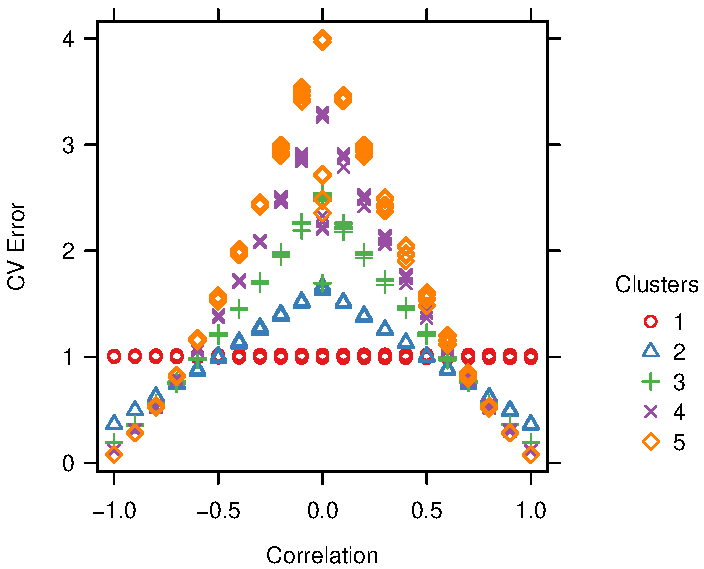
\includegraphics[width=25pc]{demo/nullcorr/equal.pdf}
\caption{Cross-validation error on $10$ replicates, with the number of
clusters $k$ ranging from $1$ to $5$.  Data is generated from two-dimensional
multivariate normal distribution with correlation $\rho$.  The Gabriel
cross-validation criterion chooses the correct answer $k = 1$ whenever
$\rho < 0.5$; the criterion chooses $k = 2$ clusters whenever $|\rho| > 0.5$.}
\label{fig:nullcorr-equal}
\end{figure}


\bibliography{references}
\bibliographystyle{apalike}
\end{document}
